% concatenated from Bollati-Olguin-Tarzia-Arxiv.tex
%  LaTeX support: latex@mdpi.com 
%  For support, please attach all files needed for compiling as well as the log file, and specify your operating system, LaTeX version, and LaTeX editor.

%=================================================================
\documentclass[11pt]{article}

\usepackage[a4paper,left=2cm,right=2cm,top=2.5cm,bottom=2.5cm]{geometry}

\usepackage{float}


\usepackage{amsmath,amssymb,amsthm}




\usepackage{hyperref}
\newcommand{\br}{\mathbb R}
\newcommand{\uu}{\text{u}}
\usepackage{color}
\newcommand{\dee}{d}
\newcommand{\bint}{\displaystyle\int}
\newcommand{\biint}{\displaystyle\iint}
\newcommand{\biiint}{\displaystyle\iiint}
\usepackage[utf8]{inputenc}
\usepackage{tikz}
\usetikzlibrary{matrix}
\usepackage[all]{xy}
\usepackage{tabularx}
\newcommand\pder[2][]{\ensuremath{\tfrac{\partial#1}{\partial#2}}}

\newtheorem{Lemma}{Lemma}
\newtheorem{Remark}{Remark}
\usepackage{booktabs}
%\numberwithin{lemma}{section}
%\documentclass[preprints,article,submit,pdftex,moreauthors]{Definitions/mdpi} 
% For posting an early version of this manuscript as a preprint, you may use ''preprints'' as the journal. Changing ''submit'' to ''accept'' before posting will remove line numbers.

% Below journals will use APA reference format:
% admsci, aieduc, behavsci, businesses, econometrics, economies, education, ejihpe, famsci, games, humans, ijcs, ijfs, journalmedia, jrfm, jsam, languages, peacestud, psycholint, publications, tourismhosp, youth

% Below journals will use Chicago reference format:
% arts, genealogy, histories, humanities, jintelligence, laws, literature, religions, risks, socsci

%--------------------
% Class Options:
%--------------------
%----------
% journal
%----------
% Choose between the following MDPI journals:
% accountaudit, acoustics, actuators, addictions, adhesives, admsci, adolescents, aerobiology, aerospace, agriculture, agriengineering, agrochemicals, agronomy, ai, aichem, aieduc, aieng, aimater, aimed, aipa, air, aisens, algorithms, allergies, alloys, amh, analog, analytica, analytics, anatomia, anesthres, animals, antibiotics, antibodies, antioxidants, applbiosci, appliedchem, appliedmath, appliedphys, applmech, applmicrobiol, applnano, applsci, aquacj, architecture, arm, arthropoda, arts, asc, asi, astronautics, astronomy, atmosphere, atoms, audiolres, automation, axioms, bacteria, batteries, bdcc, behavsci, beverages, biochem, bioengineering, biologics, biology, biomass, biomechanics, biomed, biomedicines, biomedinformatics, biomimetics, biomolecules, biophysica, bioresourbioprod, biosensors, biosphere, biotech, birds, blockchains, bloods, blsf, brainsci, breath, buildings, businesses, cancers, carbon, cardiogenetics, cardiovascmed, catalysts, cells, ceramics, challenges, chemengineering, chemistry, chemosensors, chemproc, children, chips, cimb, civileng, cleantechnol, climate, clinbioenerg, clinpract, clockssleep, cmd, cmtr, coasts, coatings, colloids, colorants, commodities, complexities, complications, compounds, computation, computers, condensedmatter, conservation, constrmater, cosmetics, covid, crops, cryo, cryptography, crystals, csmf, ctn, culture, curroncol, cyber, dairy, data, ddc, dentistry, dermato, dermatopathology, designs, devices, dhi, diabetology, diagnostics, dietetics, digital, disabilities, diseases, diversity, dna, drones, dynamics, earth, ebj, ecm, ecologies, econometrics, economies, edm, education, eesp, ejihpe, electricity, electrochem, electronicmat, electronics, encyclopedia, endocrines, energies, eng, engproc, entomology, entropy, environments, environremediat, epidemiologia, epigenomes, esa, est, famsci, fermentation, fibers, fintech, fire, fishes, fluids, foods, forecasting, forensicsci, forests, fossstud, foundations, fractalfract, fuels, future, futureinternet, futurepharmacol, futurephys, futuretransp, galaxies, games, gases, gastroent, gastrointestdisord, gastronomy, gels, genealogy, genes, geographies, geohazards, geomatics, geometry, geosciences, geotechnics, geriatrics, germs, glacies, grasses, green, greenhealth, gucdd, hardware, hazardousmatters, healthcare, hearts, hemato, hematolrep, hep, heritage, higheredu, highthroughput, histories, horticulturae, hospitals, humanities, humans, hydrobiology, hydrogen, hydrology, hydropower, hygiene, idr, iic, ijcs, ijem, ijerph, ijfs, ijgi, ijmd, ijms, ijns, ijom, ijpb, ijt, ijtm, ijtpp, ime, immuno, informatics, information, infrastructures, inorganics, insects, instruments, inventions, iot, j, jaestheticmed, jal, jcdd, jcm, jcp, jcrm, jcs, jcto, jdad, jdb, jdream, jemr, jeta, jfb, jfmk, jgbg, jgg, jimaging, jintelligence, jlpea, jmahp, jmmp, jmms, jmp, jmse, jne, jnt, jof, joi, joitmc, joma, jop, joptm, jor, journalmedia, jox, jpbi, jphytomed, jpm, jrfm, jsam, jsan, jtaer, jvd, jzbg, kidneydial, kinasesphosphatases, knowledge, labmed, laboratories, lae, land, languages, laws, life, lights, limnolrev, lipidology, liquids, literature, livers, logics, logistics, lubricants, lymphatics, machines, macromol, magnetism, magnetochemistry, make, marinedrugs, materials, materproc, mathematics, mca, measurements, medicina, medicines, medsci, membranes, merits, metabolites, metals, meteorology, methane, metrics, metrology, micro, microarrays, microbiolres, microelectronics, micromachines, microorganisms, microplastics, microwave, minerals, mining, mmphys, modelling, molbank, molecules, mps, msf, mti, multimedia, muscles, nanoenergyadv, nanomanufacturing, nanomaterials, ncrna, ndt, network, neuroglia, neuroimaging, neurolint, neurosci, nitrogen, notspecified, nursrep, nutraceuticals, nutrients, obesities, occuphealth, oceans, ohbm, onco, optics, oral, organics, organoids, osteology, oxygen, pandemics, parasites, parasitologia, particles, pathogens, pathophysiology, peacestud, pediatrrep, pets, pharmaceuticals, pharmaceutics, pharmacoepidemiology, pharmacy, philosophies, photochem, photonics, phycology, physchem, physics, physiologia, plants, plasma, platforms, pollutants, polymers, polysaccharides, populations, poultry, powders, precipitation, precisoncol, preprints, proceedings, processes, prosthesis, proteomes, psf, psychiatryint, psychoactives, psycholint, publications, purification, quantumrep, quaternary, qubs, radiation, rdt, reactions, realestate, receptors, recycling, regeneration, religions, remotesensing, reports, reprodmed, resources, rheumato, risks, rjpm, robotics, rsee, ruminants, safety, sci, scipharm, sclerosis, seeds, sensors, separations, sexes, shi, signals, sinusitis, siuj, skins, smartcities, sna, societies, socsci, software, soilsystems, solar, solids, spectroscj, sports, standards, stats, std, stratsediment, stresses, surfaces, surgeries, suschem, sustainability, symmetry, synbio, systems, tae, targets, taxonomy, technologies, telecom, test, textiles, thalassrep, therapeutics, thermo, timespace, tomography, tourismhosp, toxics, toxins, tph, transplantology, transportation, traumacare, traumas, tri, tropicalmed, universe, urbansci, uro, vaccines, vehicles, venereology, vetsci, vibration, virtualworlds, viruses, vision, waste, water, welding, wem, wevj, wild, wind, women, world, youth, zoonoticdis

%---------
% article
%---------
% The default type of manuscript is ''article'', but can be replaced by: 
% abstract, addendum, article, benchmark, book, bookreview, briefcommunication, briefreport, casereport, changes, clinicopathologicalchallenge, comment, commentary, communication, conceptpaper, conferenceproceedings, correction, conferencereport, creative, datadescriptor, discussion, entry, expressionofconcern, extendedabstract, editorial, essay, erratum, fieldguide, hypothesis, interestingimages, letter, meetingreport, monograph, newbookreceived, obituary, opinion, proceedingpaper, projectreport, reply, retraction, review, perspective, protocol, shortnote, studyprotocol, supfile, systematicreview, technicalnote, viewpoint, guidelines, registeredreport, tutorial,  giantsinurology, urologyaroundtheworld
% supfile = supplementary materials

%----------
% submit
%----------
% The class option ''submit'' will be changed to ''accept'' by the Editorial Office when the paper is accepted. This will only make changes to the frontpage (e.g., the logo of the journal will get visible), the headings, and the copyright information. Also, line numbering will be removed. Journal info and pagination for accepted papers will also be assigned by the Editorial Office.

%------------------
% moreauthors
%------------------
% If there is only one author the class option oneauthor should be used. Otherwise use the class option moreauthors.

%---------
% pdftex
%---------
% The option pdftex is for use with pdfLaTeX. Remove ''pdftex'' for (1) compiling with LaTeX & dvi2pdf (if eps figures are used) or for (2) compiling with XeLaTeX.

%=================================================================
% MDPI internal commands - do not modify
%\firstpage{1} 


%=================================================================
% Full title of the paper (Capitalized)




\title{Explicit Discrete Solution for Some Optimization Problems and Estimations with Respect to the Exact Solution}




\author{
Julieta Bollati$^{1,2}$, Mariela Olguín$^{3}$, Domingo A. Tarzia$^{1,2}$ \\
\small {{$^1$} Depto. Matem\'atica, FCE, Univ. Austral, Paraguay 1950} \\
\small {{$^2$} CONICET, Argentina} \\
\small {{$^3$} Departamento de
Matem\'atica, EFB-FCEIA, Univ. Nacional de Rosario} \\
\small {S2000FZF Rosario, Argentina.}\\
%\small{Email: jbollati@austral.edu.ar, mcolguin@fceia.unr.edu.ar,dtarzia@austral.edu.ar,}\\
}




%
\date{}

\begin{document}
\maketitle
\pagestyle{empty}
\abstract{We consider two steady-state heat conduction systems called, $S$ and $S_\alpha$, in a multidimensional bounded domain $D$  for the Poisson equation with source energy $g$.
In one system, we impose mixed boundary conditions (temperature $b$ on the boundary $\Gamma_1$, heat flux $q$ on $\Gamma_2$ and an adiabatic condition on $\Gamma_3$). In the other system,  the condition on $\Gamma_1$ is replaced by a  convective heat flux condition with coefficient $\alpha$. 
For each of these systems, we consider three associated optimization problems $(P_{i})$ and $(P_{i\alpha })$, $i=1,2,3$, where the variable is the source energy $g$, the heat flux $q$ and the environmental temperature $b$, respectively. 
In the particular case where $D$ is a rectangle, the explicit continuous optimization variables and the corresponding state of the systems are known. 
In the present work, by using a finite difference scheme, we obtain the discrete systems $({S^h})$ and ${(S^h_\alpha)}$ and discrete optimization problems ${(P^h_i)}$ and ${(P^h_{i \alpha})}$, $i=1,2,3$, where $h$ is the space step in the discretization. Explicit discrete solutions are found, and  convergence and estimation errors results are proved when $h$ goes to zero and when $\alpha$ goes to infinity. 
Moreover, some numerical simulations are provided in order to test theoretical results. Finally, we note that the use of a three-point finite-difference approximation for the Neumann or Robin boundary condition at the boundary improves the global order of convergence from $O(h)$ to $O(h^2)$.
}

% Keywords
\smallskip
\noindent {\it Keywords:}  Optimal control, finite difference, Explicit solutions. 

% The fields PACS, MSC, and JEL may be left empty or commented out if not applicable
%\PACS{J0101}
\smallskip
\noindent {\it 2000 AMS Subject Classification}{35C05; 49J20; 49K20; 49M25; 65N15; 65N30 %MDPI: We complete this section, please confirm.
%%% It is ok
}
%\JEL{}

%%%%%%%%%%%%%%%%%%%%%%%%%%%%%%%%%%%%%%%%%%
% Only for the journal Diversity
%\LSID{\url{http://}}

%%%%%%%%%%%%%%%%%%%%%%%%%%%%%%%%%%%%%%%%%%
% Only for the journal Applied Sciences
%\featuredapplication{Authors are encouraged to provide a concise description of the specific application or a potential application of the work. This section is not mandatory.}
%%%%%%%%%%%%%%%%%%%%%%%%%%%%%%%%%%%%%%%%%%

%%%%%%%%%%%%%%%%%%%%%%%%%%%%%%%%%%%%%%%%%%
% Only for the journal Data
%\dataset{DOI number or link to the deposited data set if the data set is published separately. If the data set shall be published as a supplement to this paper, this field will be filled by the journal editors. In this case, please submit the data set as a supplement.}
%\datasetlicense{License under which the data set is made available (CC0, CC-BY, CC-BY-SA, CC-BY-NC, etc.)}

%%%%%%%%%%%%%%%%%%%%%%%%%%%%%%%%%%%%%%%%%%
% Only for the journal BioTech, Fishes, Neuroimaging and Toxins
%\keycontribution{The breakthroughs or highlights of the manuscript. Authors can write one or two sentences to describe the most important part of the paper.}

%%%%%%%%%%%%%%%%%%%%%%%%%%%%%%%%%%%%%%%%%%
% Only for the journal Encyclopedia
%\encyclopediadef{For entry manuscripts only: please provide a brief overview of the entry title instead of an abstract.}

%%%%%%%%%%%%%%%%%%%%%%%%%%%%%%%%%%%%%%%%%%
% Different journals have different requirements. Please check the specific journal guidelines in the ''Instructions for Authors'' on the journal's official website.
%\addhighlights{yes}
%\renewcommand{\addhighlights}{%
%
%\noindent The goal is to increase the discoverability and readability of the article via search engines and other scholars. Highlights should not be a copy of the abstract, but a simple text allowing the reader to quickly and simplified find out what the article is about and what can be cited from it. Each of these parts should be devoted up to 2~bullet points.\vspace{3pt}\\
%\textbf{What are the main findings?}
% \begin{itemize}[labelsep=2.5mm,topsep=-3pt]
% \item First bullet.
% \item Second bullet.
% \end{itemize}\vspace{3pt}
%\textbf{What are the implications of the main findings?}
% \begin{itemize}[labelsep=2.5mm,topsep=-3pt]
% \item First bullet.
% \item Second bullet.
% \end{itemize}
%}


%%%%%%%%%%%%%%%%%%%%%%%%%%%%%%%%%%%%%%%%%%


%%%%%%%%%%%%%%%%%%%%%%%%%%%%%%%%%%%%%%%%%%
\section{Introduction}\label{intro}
%%=================================


   We consider a multidimensional bounded domain $\Omega \subset \mathbb{R}^n$ whose regular boundary $\Gamma$  consists of three disjoint portions $\Gamma_i$ with $meas(\Gamma_i) > 0,$ for   $\; i=1, 2, 3$. We define two~stationary heat conduction problems  $(S)$ and $(S_\alpha)$ with mixed boundary conditions which are given by  \eqref{ec 1.1} and \eqref{ec 1.2}, and by \eqref{ec 1.1} and \eqref{ec 1.3}, respectively: %MDPI: 1. Please check all Equations carefully, make sure that all equations is not repeat and correct. 2. Please carefully check the whole paper and make sure that same equation elements have the same format throughout the whole manuscript (italic, bold, subscript, uppercase, etc.).
 \begin{eqnarray}
 & -\Delta u=g   \quad in \quad  \Omega, &  \label{ec 1.1}\\[0.25cm]
 u\Big\vert_{\Gamma_1}=b,\qquad &-\tfrac{\partial u}{\partial n}\Big\vert_{\Gamma_2} =q , \qquad &-\tfrac{\partial u}{\partial n} \Big\vert_{\Gamma_3}=0, \label{ec 1.2}\\[0.25cm]
  -\tfrac{\partial u}{\partial n} \Big\vert_{\Gamma_1}= \alpha\,(u-b),\qquad & -\tfrac{\partial u}{\partial n} \Big\vert_{\Gamma_2}=q \qquad & -\tfrac{\partial u}{\partial n}\Big\vert_{\Gamma_3} =0 ,\label{ec 1.3}
\end{eqnarray}   
   %  \begin{equation}  \label{ec 1.1}
  %    -\Delta u=g   \,\, in \,\,  \Omega, 
  % \end{equation}
   % \begin{equation}  \label{ec 1.2}
    %   u=b \quad on \quad \Gamma_1,\qquad\quad -\tfrac{\partial u}{\partial n} =q \quad on \quad  \Gamma_2, \quad\qquad -\tfrac{\partial u}{\partial n} =0 \quad on \quad \Gamma _3,
    %\end{equation}
    %\begin{equation}  \label{ec 1.3}
    %    -\tfrac{\partial u}{\partial n} = \alpha\,(u-b)\quad on\quad \Gamma_1, \quad\quad -\tfrac{\partial u}{\partial n} =q \quad on \quad  \Gamma_2, \quad\qquad -\tfrac{\partial u}{\partial n} =0 \quad on \quad \Gamma_3,
    %\end{equation}
 
\noindent where $g$ is the internal energy of the system in $\Omega$, $b>0$ the environmental temperature  on $\Gamma_1$, $q$ is the heat flux on $\Gamma_2$ and, $\alpha>0$ is the convective heat coefficient on $\Gamma_1.$ We assume that $g \in H= L^2(\Omega)$, $q\in Q=L^2(\Gamma_2)$ and $b \in B= H^{1/2}(\Gamma_1).$  These problems correspond to stationary Stefan problems ~\cite{TaTa1989,Ta1996}.
   Notice that mixed boundary conditions play an important role in several applications, e.g., heat conduction and electric potential problems~\cite{HaMe2009}. 

  
The variational formulation of the  elliptic problems {$(S)$ and $(S_\alpha)$, corresponding to} \eqref{ec 1.1}, \eqref{ec 1.2} and \eqref{ec 1.1}, \eqref{ec 1.3}, {respectively,} can be found  in~\cite{GaTa2003,GaTa2008,TaTa1989}. In general,  solutions of mixed elliptic boundary value problems {are not very} regular~\cite{Gr1985}, but there are cases in which they are regular~\cite{AzKr1982,LaCaBr2008,Sh1968}. Other theoretical optimization problems on the subject have been {studied} in~\cite{Hi2005,WaWa2011}. 
 
We define the optimization problems $(P_i)$ and $(P_{i\,\alpha})$ $i=1,2,3$, associated to the systems $(S)$ and $(S_\alpha)$, respectively (see~\cite{Ba1984,GaTa2003,Li1968,NeSpTi2006,Tr2010}). 

The distributed optimization problems $(P_1)$ and $(P_{1\alpha})$ on the constant internal energy $g$ are formulated as:
\begingroup
\addtolength{\jot}{0.5em}
\begin{align}
& \text{ find }\quad g_{op}\in \mathbb{R}\quad\text{ such that }\quad
J_{1}(g_{op})=\min\limits_{g\in \mathbb{R}} \text{ }J_{1}(g)
\label{PControlJ1} \\
& \text{find }\quad g_{{\alpha}_{op}}\in \mathbb{R}\quad\text{ such that
}\quad J_{1\alpha}(g_{{\alpha}_{op}})=\min\limits_{g\in \mathbb{R}} \text{
}J_{1\alpha}(g)  \label{PControlalfaJ1}
\end{align}
\endgroup
where $J_{1}:\mathbb{R}{\rightarrow}{\Bbb R}_{0}^{+}$ and
$J_{1\alpha}:\mathbb{R}{\rightarrow}{\Bbb R}_{0}^{+}$ are given by
\begin{equation} \label{J1-J1alpha}
J_{1}(g)=\frac{1}{2}\left\|u_{g}-z_{d}\right\|
_{H}^{2}+\frac{M_{1}}{2}\left\| g\right\|_{H}^{2},\qquad J_{1\alpha}(g)=\frac{1}{2}\left\|u_{\alpha
g}-z_{d}\right\| _{H}^{2}+\frac{M_{1}}{2}\left\| g\right\|_{H}^{2}
\end{equation}
with $M_{1}\in\mathbb{R}^+$ and $z_{d}\in \mathbb{R}$. { For each $g \in \mathbb{R}$, $u_g$ and $u_{\alpha g}$ denote the unique solutions to the systems $(S)$ and $(S_\alpha)$, respectively, for given data $q \in \mathbb{R}$ and $b \in \mathbb{R}$.  }
{ Here and throughout this section, $\|\cdot\|_H$ denotes the standard $L^2(\Omega)$ norm.}







The boundary optimization problems $(P_2)$ and $(P_{2\alpha})$ on the constant heat flux $q$ on $\Gamma_{2}$ are defined as:
\begingroup
\addtolength{\jot}{0.5em}
\begin{align}
& \text{find }\quad q_{op}\in \mathbb{R}\quad\text{ such that }\quad
J_{2}(q_{op})=\min\limits_{q\in \mathbb{R}}\,J_{2}(q) \label{PControlJ2} \\
& \text{find }\quad q_{{\alpha}_{op}}\in \mathbb{R}\quad\text{ such that
}\quad J_{2\alpha}(q_{{\alpha}_{op}})=\min\limits_{q\in\mathbb{R}}\,J_{2\alpha}(q)  \label{PControlalfaJ2}
\end{align}
\endgroup
where 
$J_{2}:\mathbb{R}{\rightarrow}{\Bbb R}_{0}^{+}$ and
$J_{2\alpha}:\mathbb{R}{\rightarrow}{\Bbb R}_{0}^{+}$ are given by
\begin{equation}\label{J2-J2alpha}
J_{2}(q)=\frac{1}{2}\left\| u_{q}-z_{d}\right\|
_{H}^{2}+\frac{M_{2}}{2}\left\| q\right\|_{Q}^{2}, \qquad
J_{2\alpha}(q)=\frac{1}{2}\left\| u_{\alpha
q}-z_{d}\right\| _{H}^{2}+\frac{M_{2}}{2}\left\| q\right\|_{Q}^{2}
\end{equation}
with $M_2\in\mathbb{R}^+$ and $z_d\in
\mathbb{R}$. For each $q\in\mathbb{R}$,  we denote with $u_{q}$ and $u_{\alpha q}$  the unique solutions to the
systems $(S)$ and $(S_\alpha)$ respectively,  for data $g\in \mathbb{R}$ and $b\in \mathbb{R}$. 
{ Here and throughout this section, $\|\cdot\|_Q$ denotes the standard $L^2(\Gamma_2)$ norm.}

The boundary optimization problems $(P_3)$ and $(P_{3\alpha})$ on the constant temperature $b$ in an external neighborhood of $\Gamma_{1}$ are set as
\begingroup
\addtolength{\jot}{0.5em}
\begin{align}
& \text{find }\quad b_{op}\in \mathbb{R} \quad\text{ such
that }\quad J_{3}(b_{op})=\min\limits_{b\in
\mathbb{R}}\,J_{3}(b)
\label{PControlJ3} \\
& \text{find }\quad b_{{\alpha}_{op}}\in
\mathbb{R}\quad\text{ such that }\quad
J_{3\alpha}(b_{{\alpha}_{op}})=\min\limits_{b\in
\mathbb{R}}\,J_{3\alpha}({b})  \label{PControlalfaJ3}
\end{align}
\endgroup
where $J_{3}:\mathbb{R}{\rightarrow}{\Bbb R}_{0}^{+}$ and
$J_{3\alpha}:\mathbb{R}{\rightarrow}{\Bbb R}_{0}^{+}$, given by
\begin{equation}\label{J3-J3alpha}
J_{3}(b)=\frac{1}{2}\left\| u_{b}-z_{d}\right\|
_{H}^{2}+\frac{M_{3}}{2}\left\| b\right\|_{B}^{2},\qquad J_{3\alpha}(b)=\frac{1}{2}\left\| u_{\alpha b}-z_{d}\right\|
_{H}^{2}+\frac{M_{3}}{2}\left\| b\right\|_{B}^{2}
\end{equation}
\noindent with $M_3\in\mathbb{R}^+$ and $z_d\in \mathbb{R}$. For every $b\in\mathbb{R}$, the functions $u_{b}$ and $u_{\alpha b}$ are the unique solutions of  systems $(S)$ and $(S_\alpha)$ respectively, for data $g\in \mathbb{R}$ and $q\in\mathbb{R}$. 
{Here and throughout this section, $\|\cdot\|_B$ denotes the standard norm in $B=H^{1/2}(\Gamma_1)$.
}



{ In~\cite{BoGaTa2020}, explicit solutions to the continuous systems $(S)$ and $(S_\alpha)$ were derived, together with  the associated optimization problems $(P_i)$ and $(P_{i\alpha})$ for $i=1,2,3$, in the particular case where the domain is a rectangle. These explicit solutions serve as a rigorous benchmark for assessing the accuracy and reliability of numerical methods.}
  
{The aim of this paper is three-fold: 
(i) to obtain explicit solutions to the systems $(S)$ and $(S_\alpha)$ in a rectangular domain; 
(ii) to derive explicit discrete solutions for the optimization problems $(P_i)$ and $(P_{i\alpha})$, $i=1,2,3$, using finite difference methods; 
and (iii) to estimate the order of convergence of the discrete solutions by comparison with the exact explicit ones.}
 
It is worth mentioning that there are several articles available in the literature that obtain explicit  discrete  solutions of some optimization problems~\cite{An1968,ArMoUg2011}. 
For example, in~\cite{LaSc2023},  exact formulas are derived for the solution of an optimal boundary control problem governed by the one-dimensional heat equation where the control function  measures the distance of the final state from the target. In~\cite{YaSu2023} a finite element approximation is applied for some kind of parabolic optimal control problems with Neumann boundary conditions. Some numerical experiments are carried out setting a rectangular domain.


This paper is organized as follows: in Section~\ref{sec2} we obtain the discrete explicit solution to the systems $(S)$ and $(S_\alpha)$ by the finite difference method. In Section~\ref{sec3}, we obtain explicit discrete solutions to the discrete distributed optimization problems associated with $(P_1)$ and $(P_{1\alpha})$, respectively, where the  variable is the internal energy $g$. 
In Section~\ref{sec4}, we define  discrete boundary optimization problems where the variable is the heat flux $q$, associated with $(P_2)$ and $(P_{2\alpha})$, respectively, obtaining the discrete explicit  solutions. In the same manner, in Section~\ref{sec5}, we derive explicit discrete solutions to the discrete boundary optimal control problems associated with $(P_3)$ and $(P_{3\alpha})$, respectively, where the optimization variable is $b$.  In all cases, when the step discretization goes to zero, convergence results are obtained by also estimating the order of convergence of the approximate solutions.
In Section~\ref{sec6}, we carry out some numerical simulations  in order to illustrate the theoretical convergence results obtained in the previous sections. Finally,  in Section~\ref{sec7}, we analyze the order of convergence of the discrete systems associated with $(S)$ and $(S_\alpha)$ by considering a modified approximation of the Neumann boundary condition on $\Gamma_2$, which leads to an improved convergence order.
 
 
{The explicit continuous solutions of the systems and the associated optimal control problems in a rectangular domain are already available in the literature; in particular, they are given in~\cite{BoGaTa2020}. 

The novelty of the present work can be summarized as follows: 
(i) the derivation of explicit discrete solutions for the state and the control variables; 
(ii) a rigorous analysis of the convergence of the discrete solutions, including the estimation of their orders of convergence; 
and (iii) an improved approximation of the boundary conditions in the discrete framework.}
% El objetivo de este trabajo es el de hallar las soluciones discretas expl\'icitas que aproximan
%    a las soluciones continuas de los sistemas $(S)$ y $(S_\alpha)$ y de los problemas de control \'optimo
%    de frontera asociados $(P)$ y $(P_\alpha)$, descriptos por (\ref{ec 1}, \ref{ec 2}), (\ref{ec 1}, \ref{ec 3}), (\ref{ec 6}, \ref{ec 8}) y
%    (\ref{ec 7}, \ref{ec 9}) respectivamente considerando un dominio $\Omega$ particular de forma
%    rectangular en el plano y obtener estimaciones de error.
%  pendiente%%%%%%%%%%%%%%%%%%%%%%%%%%%%%%%%%%%%%%%%%%%%%%%%%%%
%    En el trabajo~\cite{Gariboldi08} se obtuvieron resultados de existencia y unicidad
%    para el sistema $S$ y para el problema de control \'optimo continuo $(P)$ en determinado espacio
%    y en el trabajo {~\cite{Tarzia16} se realiz\'o el an\'alisis num\'erico correspondiente.
%    Adem\'as, en~\cite{Bollati17} se obtuvieron las soluciones expl\'icitas para los problema de control
%    continuo $(P)$ y $(P_\alpha)$ para un dominio rectangular en el plano, como as\'i tambi\'en para los
%    sistemas $(S)$ y $(S_\alpha)$ correspondientes.
% 
%    El objetivo de este trabajo es el de hallar las soluciones discretas expl\'icitas que aproximan
%    a las soluciones continuas de los sistemas $(S)$ y $(S_\alpha)$ y de los problemas de control \'optimo
%    de frontera asociados $(P)$ y $(P_\alpha)$, descriptos por (\ref{ec 1}, \ref{ec 2}), (\ref{ec 1}, \ref{ec 3}), (\ref{ec 6}, \ref{ec 8}) y
%    (\ref{ec 7}, \ref{ec 9}) respectivamente considerando un dominio $\Omega$ particular de forma
%    rectangular en el plano y obtener estimaciones de error. Con este fin, en la Secci\'on 2, siguiendo lo hecho 
%    en \cite {Bollati17} y utilizando el m\'etodo de diferencias finitas~\cite{Crank84} con $h$ el par\'ametro de la
%    discretizaci\'on se tiene, de manera expl\'icita, la soluci\'on discreta del sistema lineal de ecuaciones 
%    que resulta, llamado $(S_h)$. Adem\'as, se establece la funci\'on costo discreto, llamado as\'i dado
%    que se define en funci\'on de la soluci\'on del sistema $(S_h)$. Se plantea la familia de problemas de control
%    \'optimo discreto $(P_h)$, dependiente del par\'ametro $h$ y nuevamente se analizan estimaciones de error.
%    En la Secci\'on 3, se trabaja en forma similar para establecer la discretizaci\'on del sistema $(S_\alpha)$ 
%    y del problema $(P_\alpha)$ y a la vez obtener resultados de convegencia cuando el par\'ametro $h$ tiende a cero.
%    Por \'ultimo, en la Secci\'on 4, los resultados te\'oricos se chequean con resultados num\'ericos para distintos
%    valores del paso espacial $h$ cuando $h$ tiende a cero. 

%\bigskip

%These explicit discrete solutions could be used to check numerical calculations  for conditions in general domains.

\section{Discrete Systems for \boldmath{$(S)$} and \boldmath{$(S_\alpha)$}}\label{sec2} %2

In this section we obtain the discrete explicit solutions to the  systems $(S)$ and $(S_\alpha)$ in a rectangular  domain in the plane  $\Omega = (0, x_0) \times (0, y_0)$ with $x_0>0$ and $y_0 > 0$. Its boundaries $\Gamma_i$ for $i=1,2,3$  are defined by:


     \[\Gamma_1= \{(0,y):\, y\in (0,y_0]\}, \quad \Gamma_2= \{(x_0,y):\, y\in (0,y_0]\} \]
      and
 \[ \Gamma_3= \{(x,0):\, x\in [0,x_0]\} \cup \{(x,y_0):\, x\in [0,x_0]\}.\]
    
According to~\cite{BoGaTa2020}, the continuous solutions, in $\Omega$, for the systems $(S)$ and $(S_\alpha)$ defined by \eqref{ec 1.1}, \eqref{ec 1.2}
and \eqref{ec 1.1}, \eqref{ec 1.3} are given by:
\begin{equation}\label{Def: u y ualpha}
\begin{array}{ll}
 u (x, y) = -\tfrac{1}{2} g x^2 + (g x_0 - q) x +b, \qquad \forall \;\; (x,y) \in \Omega   \\ 
 \\
 u_\alpha (x, y)= -\tfrac{1}{2} g x^2 + (g x_0 - q) x + \tfrac{1}{\alpha} (g\,x_0 - q) +b ,\qquad \forall \;\; (x,y) \in \Omega. 
 \end{array}
 \end{equation}

 
As %MDPI: Please check if no indent format should be keep in whole text.
a consequence of the symmetry of domain $\Omega$ {and the boundary conditions},  the solutions $u$ and $u_\alpha$ of systems $(S)$ and $(S_\alpha)$ are independent of variable $y$, and therefore, we  work  with one-dimensional problems.
      

      
      Given $n \in \mathbb{N}$, we define:
          \begin{equation} \label{ec 2.1}
    	    h= \tfrac{x_0}{n}; \quad x_i = (i-1) \,h, \text{ for } i=1,\ldots, n+1, \quad {u^h_i} \approx  u(x_i, y)  \text{ for } i=2, \ldots,n+1.
          \end{equation}
    
        
 {
Here, $n$ is the number of subintervals of $[0,x_0]$, $h$ is the uniform mesh size, $u^h_1=b$, and $u^h_i$ denotes the discrete approximation of the temperature at the node $x_i$, $i=2,\ldots,n+1$. Since the temperature is constant along the $y$-direction, $u^h_i$ approximates $u(x_i,y)$ for any $(x_i,y)\in\Omega$.
}

We apply the classical finite-difference method to the system $(S)$ described by \mbox{Equations} \eqref{ec 1.1} and \eqref{ec 1.2}.
Since the boundary condition on $\Gamma_1$ prescribes $u(0,y)=b$, we immediately obtain $u_1=b$.

For the interior nodes, we use the classical centered second-order finite-difference approximation:
\begin{equation}\label{aprox-deriv}
\frac{\partial^2 u}{\partial x^2}(x_i,y)\approx 
\frac{u(x_{i+1},y)-2u(x_i,y)+u(x_{i-1},y)}{h^2},
\qquad i=2,3,\ldots,n,
\end{equation}
and from {the differential equation} \eqref{ec 1.1}, {we impose that}
\begin{equation}\label{aprox-nodo-interior}
-gh^{2}= {u^h_{i+1}}-2{u^h_i}+{u^h_{i-1}},
\qquad i=2,3,\ldots,n.
\end{equation}


To incorporate the Neumann boundary condition on $\Gamma_2$,  we use a backward finite difference for the first derivative:
\begin{equation}\label{aprox-Neumann}
\frac{\partial u}{\partial x}(x_{n+1},y)\approx 
\frac{u(x_{n+1},y)-u(x_{n},y)}{h},
\end{equation}
which, using the boundary condition 
\(\frac{\partial u}{\partial x}(x_{n+1},y)=q\),
leads to {assuming that}
\begin{equation}\label{aprox-un+1}
-qh = {u^h_{n+1}} - {u^h_{n}}.
\end{equation}
{Taking into account  \eqref{aprox-nodo-interior} and \eqref{aprox-un+1}, the resulting discretization leads to the} discrete linear system ${(S^h)}$
\begin{equation}\label{sistema-tradicional}
{A\,v^h = T^h,}
\end{equation}
where ${v^h} = ({u^h_i})_{i=2,\ldots,n+1}\in\mathbb{R}^{n}$ {denotes} the vector of unknowns, $A$ is the associated tridiagonal coefficient matrix:


    					\begin{equation}\label{matrizA}
    					A=\begin{pmatrix}
-2 & 1 & 0 & \ldots & \ldots & & 0 &\\                                                                                                   
1 &-2 & 1&0 &\ldots &&0 \\
0 &1& -2 & 1&0&\ldots &0 \\
\vdots\\
0 &\ldots &0 & 1&-2 & 1 &0\\
0 &\ldots & \ldots & 0&1 & -2 & 1\\
 0 &\ldots& \ldots& \ldots &  0& -1 &1
\end{pmatrix}_{n\times n}
\end{equation} 
    and ${T^h}\in \mathbb{R}^n$ is  the vector of independent terms:
    \begin{equation}\label{vectorT}
     {T^h}= \Big(-g\,h^2 - b, -g h^2, \ldots, -g h^2, -q\,h  \Big)^t.\end{equation}
    

     
    \noindent The square matrix $A$ is invertible and its inverse matrix is given by
\[A^{-1}=\begin{pmatrix}
-1 & -1 & -1 & \ldots & \ldots & -1 & 1 &\\                                                                                                   
-1 & -2 & -2 & \ldots & \ldots & -2 & 2 &\\                                                                                                   
-1 & -2 & -3 & \ldots & \ldots & -3 & 3 &\\                                                                                                   
\vdots & \vdots & \vdots  &&& \vdots  & \vdots\\
-1& -2 & -3 &\ldots && -(n-1) & n-1\\
 -1 & -2& -3& \ldots &  &-(n-1) &n
\end{pmatrix}_{n\times n}.\]%_{n\times n}\]
Then, the linear system ${(S^h)}$ has a unique solution:
$$ {u^h_{i}}= b+  h^2g  \left( (i-1) \;n-\tfrac{i(i-1)}{2}\right)-(i-1) hq,\quad i=2 ,\ldots, n+1.$$   
As $n=\tfrac{x_0}{h}$ {and $u^h_1=b$}, it follows that:
    \[ \qquad\quad {u^h_i} = b + (i-1) \,h \,(g\,x_0-q) -  h^2 g \, \tfrac{\,i(i-1)\,}{2},\quad i=1, \ldots, n+1. \]
    
 
    
    
 Then, the continuous solution $u(x,y)$ of system $(S)$ can be approximated by the piecewise linear interpolant {$u^h(x,y)$} obtained from the nodal values computed by the finite difference scheme. More precisely, we define
          \begin{equation}\label{Def uh}
    	    {u^h}(x, y)= (g x_0  - q - h\, g\, i) x + h^2 g \Big(\tfrac{i(i-1)}{2}\Big) + b,\quad x \in [x_i, \,x_{i+1}], \,   \;y\in [0, y_0], 
          \end{equation}
with $i=1, \ldots , n.$



The following lemma{ shows that the discrete solution ${u^h}$ provides a first-order accurate approximation of the exact solution $u$ and its derivative with respect to $x$.}

  \begin{Lemma}\label{Cota u uh} $ $
    \begin{enumerate}   	
\item[(a)]  For every %MDPI: Based on our rules, statement should be label as 1, 2, 3... So we renumbered all statement and their citation in main text, please confirm whole text.
 {grid point} $(x_i,y)$ with $i=1,\ldots, n+1$, $y\in[0,y_0]$, {the following comparison holds}: 
    				\begin{itemize}
    						\item [(i)] if $g > 0$  then ${ u^h}(x_i,y) \leq u(x_i,y)$.
 
    						\item [(ii)] if $g < 0,$ then ${ u^h}(x_i,y) \geq u(x_i,y)$.
    				\end{itemize}    
    				
\item[(b)]  {The approximation error satisfies first-order estimates in the $H$-norm, namely,}
    		\[\lVert u-{ u^h} \rVert _H \leq  C_1\,h, \qquad \text{and}\qquad
\lVert \pder[u]{x}-\pder[{u^h}]{x} \rVert _H \leq \widetilde{C_{1}}\, h, \]
    		where {the  constants $C_1$ and $\widetilde{C_1}$, which do not depend on $h$,  are given by }
    		$C_1= x_0\,|g| \,\sqrt{\tfrac{2}{15}x_0\, y_0}$ and $\widetilde{C_{1}}= |g|\sqrt{\tfrac{1}{3}x_0 \, y_0}. $
    \end{enumerate}
    
    \end{Lemma}
\begin{proof} $ $

    \begin{itemize}
     \item[(a)] From the functions $u$ and ${ u^h}$, {given by \eqref{Def: u y ualpha} and \eqref{Def uh}, respectively}, we have 
    			\[ u(x_i, y) - { u^h}(x_i,y)=   \tfrac{g\,h^2 \,(i-1)}{2}, \quad i=1, \ldots , n+1.\] 
      
     \item[(b)] From the definition of the norm in space $H$ and Formulas \eqref{Def: u y ualpha} and \eqref{Def uh} for functions $u$ and ${ u^h}$, respectively, it follows that: 
     $$\begin{array}{ll}
     ||u-{ u^h}||_{H}^2& =y_0 \displaystyle\sum\limits_{i=1}^n \bint_{x_i}^{x_{i+1}}  \big(u(x,y)-{ u^h}(x,y)\big)^2  \dee x\\ 
     \\
    &=\frac{1}{120} y_0 \, h^5\, g^2\, n^3\,\big(\frac{1}{n^2}+\frac{5}{n}+10 \big)\\ 
    \\
        &\leq \frac{2}{15}\,y_0\, h^5\, g^2\, n^3=\frac{2}{15}\, h^2 g^2 \,x_0^3\,y_0=C_1^2 h^2.
     \end{array}$$
    \end{itemize}
The norm  $||\pder[u]{x}-\pder[{u^{h}}]{x}||_{H}$ can be computed analogously.
\end{proof}

    

  We next apply the classical finite-difference method to the system $(S_\alpha)$ defined by Equations \eqref{ec 1.1} and \eqref{ec 1.3}. {For each $n\in\mathbb{N}$, we set $h=\frac{x_0}{n}$ and denote by $u^h_{\alpha,i} \approx u_\alpha(x_i,y)$ the approximate value of $u_\alpha$ at $(x_i,y)$} for $i=1,\cdots,n+1$.


The Robin boundary condition on $\Gamma_1$ is approximated by a {classical forward finite-difference scheme}, namely,
\begin{equation}
{\frac{u_\alpha(x_2,y)-u_\alpha(x_1,y)}{h}\approx \frac{\partial u_\alpha}{\partial x}(x_1,y)}.
\end{equation}
{Taking into account that $\frac{\partial u_\alpha}{\partial x}(x_1,y)
=\alpha\bigl(u_\alpha(x_1,y)-b\bigr)$, we impose that}
\begin{equation}\label{Robin-Clasica}
{\frac{{u^h_{\alpha,2}}-{u^h_{\alpha,1}}}{h}
= \alpha \bigl({u^h_{\alpha,1}}-b\bigr).}
\end{equation}

Moreover, at the interior nodes we use the approximation given in \eqref{aprox-nodo-interior}, while the Neumann boundary condition at $x_{n+1}$ is discretized according to \eqref{aprox-Neumann}.

Then, we obtain the linear system ${(S^h_{\alpha})}$:
       \[A_\alpha \, {v^h_\alpha} = {T^h_\alpha},\]
 \noindent where the vector of unknowns ${v^h_\alpha} \in  \mathbb{R}^{n+1}$ is given by ${v^h_\alpha} = ({u^h_{\alpha,i}} )_{i= 1,\ldots n+1}$,  the tridiagonal coefficient matrix  $A_\alpha$  of order $n+1$ is defined as: 
  \begin{equation}\label{matrizAalpha}
     					A_{\alpha}=\begin{pmatrix}
                                                            -(1+\alpha\,h) & 1 & 0 & \ldots & \ldots & & 0 &\\                                                                                                   
                                                             1 &-2 & 1& \\
                                                             \vdots &
                                                             \ldots & \ldots & &1 & -2 & 1\\
                                                              0 & 0& 0& \ldots &  0& -1 &1
                                                    \end{pmatrix}_{(n+1)\times (n+1)}
                                                    \end{equation}
                                                    
  \noindent and \begin{equation}\label{Talpha}
  {T^h_\alpha}= \Big(-\alpha\,b\,h, -g h^2, \ldots, -g h^2, -q\,h  \Big)^t \in  \mathbb{R}^{n+1}.
  \end{equation}
     
 \noindent It can be seen that the square matrix $A_{\alpha}$ is invertible  and its inverse matrix is given by
 
 
\begin{scriptsize}
\[A_{\alpha}^{-1}=\frac{1}{\alpha h}\begin{pmatrix}
-1 & -1 & -1 & \ldots & \ldots & -1 & 1 &\\                                                                                                   
-1 & -(1+\alpha h) & -(1+\alpha h) & \ldots & \ldots & -(1+\alpha h) & 1+\alpha h &\\                                                                                                   
-1 & -(1+\alpha h) & -(1+2\alpha h) & \ldots & \ldots &-(1+2\alpha h) & -(1+2\alpha h) &\\                                                                                                   
\vdots & \vdots & \vdots  &&& \vdots  & \vdots\\
-1& -(1+\alpha h)& -(1+2\alpha h) &\ldots && -(1+(n-1)\alpha h) & 1+(n-1)\alpha h\\
 -1 & -(1+\alpha h)& -(1+2\alpha h)& \ldots &  &-(1+(n-1)\alpha h) &1+n\alpha h
\end{pmatrix}_{(n+1)\times (n+1)}\] 
\end{scriptsize}
 
 
 
Then, the linear system ${(S^h_{\alpha})}$ has a unique solution:
\[ {u^h_{\alpha,\,i}} = (b + \tfrac{g\,x_0 - q}{\alpha}) + (i-1)  \,(g\,x_0-q)\; h - \tfrac{g}{\alpha}\,h  -   g \, \tfrac{\,i(i-1)\,}{2}\,h^2,\quad i=1, \ldots, n+1. \]
      
 {As a consequence, the continuous solution $u_{\alpha}(x, y)$ of system $(S_\alpha)$ given by \eqref{Def: u y ualpha} can be approximated in $\overline{\Omega}$ by the discrete function $u^h_{\alpha}(x, y)$, defined as the piecewise linear interpolation of the nodal values obtained from the finite-difference system $(S^h_{\alpha})$.
}
 \begin{equation}\label{ec 2.3}
     	   { u^h_{\alpha}} (x, y) = ( g\, x_0 - q - h\, g\, i) x + 
     	    b +  \tfrac{g\,x_0 - q}{\alpha} -  \tfrac{g\,h}{\alpha} +  \tfrac{i^2-i}{2} g\,h^2 ,
           \end{equation}
     	for $x \in [x_i, \,x_{i+1}], y\in [0, y_0]$, $i=1, \ldots , n.$

Notice that  ${u^h_{\alpha}(x,y)}\to u^h(x,y)$ when $\alpha\to \infty$  for every $(x,y)\in \overline{\Omega}$.



\begin{Lemma}\label{lema convergencia uhalpha a ualpha}
{Let} $u_{\alpha}$ {be}  the solution of {problem }$(S_\alpha)$, {where $\alpha>0$ is the convective heat transfer coefficient appearing in the Robin boundary condition, and let $u^h_{\alpha}$ denote its piecewise linear discrete approximation defined} in (\ref{ec 2.3}). {Then, for each mesh size}  $h$, {the following error estimates hold}:
     		\[\lVert u_\alpha-{u^h_{\alpha}}  \rVert _H \leq C_{1\alpha}\,h,\qquad \qquad \text{and}\qquad
\lVert \tfrac{\partial u_{\alpha }}{\partial x}-\tfrac{\partial {u^h_{\alpha}}}{\partial x} \rVert _H \leq \widetilde{C_{1}}\, h, \]
     		{where } $C_{1\alpha}= \lvert\,g\rvert x_0\sqrt{ x_0\,y_0 \Big( \frac{2}{15} +\frac{2}{3}\frac{1}{\alpha x_0} + \tfrac{1}{\alpha^2 x_0^2} \Big)  }$ and $\widetilde{C_{1}}= |g|\sqrt{\tfrac{1}{3}x_0 \, y_0} $ {are positive constants independent of $h$. }
     	
\end{Lemma}

\begin{proof}
{Taking into account that $u_\alpha$ and {$u^h_{\alpha}$} are given by \eqref{Def: u y ualpha} and \eqref{ec 2.3}, respectively}, we have
 $$\begin{array}{ll}
&     ||u_\alpha-{u^h_{\alpha}}||_{H}^2 =y_0 \displaystyle\sum\limits_{i=1}^n \bint_{x_i}^{x_{i+1}}  \big(u_\alpha(x,y)-{u^h_{\alpha}}(x,y)\big)^2  \dee x\\ 
    &=y_0 \, g^2 \displaystyle\sum\limits_{i=1}^n  \, \frac{h^5 i^2}{4}-\frac{h^5 i}{6}+\frac{h^5}{20}-\frac{h^4}{3 \alpha }+\frac{h^4 i}{\alpha }+\frac{h^3}{\alpha ^2}\\ 
   &= y_0\, g^2\, \Big[ h^5 n^3 \left( \frac{1}{12}+\frac{1}{24n}+\frac{1}{120n^2}\right) +\frac{h^4 n^2}{\alpha}\left( \frac{1}{2}+\frac{1}{6n}\right)+\frac{h^3n}{\alpha^2} \Big]\\
 &  \leq x_0\,  y_0\, g^2\,h^2 \, \Big( \frac{2}{15}x_0^2+\frac{2}{3} \frac{x_0}{\alpha}+\frac{1}{\alpha^2} \Big)=C_{1\alpha}^2 h^2.
     \end{array}$$
In addition, the {partial derivatives with respect to $x$} of functions $u_\alpha$ and {$u^h_{\alpha}$} are given by:
$$\pder[u_{\alpha}]{x}(x,y)=\pder[u]{x}(x,y)=-gx+gx_0-q,\qquad \forall (x,y)\in \Omega$$ 
   and
    $$\pder[{u^h_{\alpha}}]{x}(x,y)=\pder[{u^{h}}]{x}(x,y)=  g\; x_0-q-h\,g\,i, \qquad x\in [x_i,\, x_{i+1}],\quad y\in\,[0,y_0].$$
Then, the bound for $\lVert \pder[u_{\alpha}]{x}-\pder[{u^h_{\alpha}}]{x} \rVert _H$  coincides with the bound for $\lVert \pder[u]{x}-\pder[{u^h}]{x} \rVert _H$,  obtained in Lemma \ref{Cota u uh}.
\end{proof}     

\begin{Remark}
Notice that $C_{1\alpha}\to C_1$ when $\alpha\to \infty$, where $C_1$ is {the constant appearing} in Lemma~\ref{Cota u uh}. This shows that the error bound associated with the convective boundary condition converges to the one obtained for the Dirichlet problem as $\alpha \to \infty$.

\end{Remark}


 %seccion 3  
\section{Distributed Optimization Problem with Variable \boldmath{$g$}}\label{sec3}   %3
In this section we obtain  discrete optimal  solutions to the continuous optimization problem $(P_1)$ and $(P_{1\alpha})$ in the rectangular domain $\Omega$ for the case where the optimization variable is $g$.

\subsection{Discrete Problem  ${(P^h_{1})}$ Associated with $(P_1)$}\label{sec3.1}
 %3.1
 
 Taking into account that $b, \,g,\,q$ and  the desired state $z_d$  in \eqref{J1-J1alpha} are constants, according to~\cite{BoGaTa2020}, the continuous quadratic  functional cost for problem $(P_1)$ is explicitly given by:
\begin{equation} \label{J1-explicito}   
    J_1(g)= \tfrac{1}{2} x_0^3\, y_0\, q^2 \Big\{ g^2 \,\tfrac{x_0^2}{q^2} \Big(\tfrac{2}{15}  + \tfrac{M_1}{x_0^4} \Big) + g \tfrac{x_0}{q}  \Big(- \tfrac{5}{12}  + \tfrac{2}{3} \tfrac{(b- z_d)}{q x_0} \Big) + \\
    \tfrac{1}{3} - \tfrac{(b-z_d)}{q x_0} + \tfrac{(b-z_d)^2}{q^2x_0^2} \Big\}.
    \end{equation}
    
 %  Since the function $J_1(g)$ is a polynomial function  of the variable $g$, the analytic expresssion for $J_1'(g)$ is given by
 %  \begin{equation}\label{J1'}
 %  J_1'(g)=\tfrac{1}{2} x_0^3y_0 q^2\left\lbrace  \tfrac{2x_0^2}{q^2}g\left( \tfrac{2}{15}+\tfrac{M_1}{x_0^4}\right)+\tfrac{x_0}{q} \left( -\tfrac{5}{12}+\tfrac{2}{3}%\tfrac{(b-z_d)}{qx_0}\right)\right\rbrace
%   \end{equation}
    
\noindent Then, the solution to the distributed optimization problem $(P_1)$ is $g_{op}$ defined by:
     \begin{equation}\label{gop}
          g_{op} = \frac{q}{3\, x_0} \frac{\Big( \tfrac{5}{8 } -\tfrac{ (b -z_d)}{q \, x_0}\Big)}{\Big(\tfrac{2}{15} + \tfrac{M_1}{x_0^4} \Big)}
     \end{equation}
   \noindent and the continuous optimization state when $g=g_{op}$ is     
       \begin{equation}\label{ugop}
            u_{g_{op}}(x,y) = -\tfrac{1}{2} g_{op}\, x^2 + (g_{op}\, x_0 - q) x +b.
       \end{equation}        
 

We define the discrete distributed optimization problem ${(P^h_{1})}$ for the constant internal energy $g$ as 
$$ \text{ find }\quad {g^h_{op}}\in \mathbb{R}\quad\text{ such that }\quad
{J^h_1(g^h_{op})}=\min\limits_{g\in \mathbb{R}} \text{ }{J^h_{1}(g)}
$$
where the discrete cost function  ${J^h_{1}}$ is given by:
    \[{J^h_{1} }(g)=  \tfrac{1}{2} \lVert u^h_g - z_d \rVert^2_H +  \tfrac{1}{2} M_1 \lVert g \rVert ^2_{H} .\]
    {Here, $u^h_g$ denotes the discrete approximation corresponding to the internal energy $g$ (see~\eqref{Def uh}), $h$ is the discretization step defined in \eqref{ec 2.1}, $z_d$ is the desired target, and $M_1>0$ is a regularization parameter. }
    
    
    Taking into account that the variable $g$ is constant results in:
     
\begin{equation}
{J^h_{1}} (g)= \tfrac{1}{2} y_0 \Big\{M_1\,g^2 \,x_0 + \, \sum_{i=1}^n \, \int_{x_i}^{x_{i+1}} \left({u^h_g (x,y) }- z_d\right)^2 \,\dee x \Big \}
\end{equation}
 and from algebraic work, it follows that
\begin{equation}\label{J1h-explicito}   \begin{array}{rl}
    {J^h_{1}(g)}&= \frac{1}{2} x_0^3\, y_0 \,q^2 \Bigg\{g^2 \tfrac{x_0^2}{q^2} \Big[\frac{2}{15}+\tfrac{M_1}{x_0^4}+\frac{1}{180} \tfrac{h^4}{x_0^4}+\frac{1}{24}\tfrac{h^3}{x_0^3}+\frac{1}{36}\tfrac{h^2}{x_0^2}-\frac{5 }{24} \tfrac{h}{x_0}\Big] \\[0.35cm]
&    + g\,\tfrac{x_0}{q} \Big[- \frac{5}{12}+ \frac{2}{3} \tfrac{(b-z_d)}{q x_0}   + \tfrac{h}{x_0}  \Big( \frac{1}{3} +  \frac{1}{12}\tfrac{h}{x_0} \Big) -  \tfrac{h}{x_0} \,\tfrac{(b-z_d)}{qx_0} \Big(  \frac{1}{2} + \tfrac{1}{6}\tfrac{h}{x_0} \Big) \Big] \\[0.35cm]
 &   + \frac{1}{3} - \tfrac{(b-z_d)}{q\,x_0}  + \tfrac{(b-z_d)^2 }{q^2\,x_0^2}\Bigg\}. \end{array}
 \end{equation}
    

    
\begin{Lemma}    \label{Lema:J1(g)-J1h(g)}
{For any given internal energy $g \in \mathbb{R}$, the following estimate holds for the discrete cost functional $J^h_{1}$:}
    \begin{equation}\label{ec 3.3}
       \lvert J_1(g) - {J^h_{1}}(g)\rvert  \approx C_2 \, h 
    \end{equation}
   where  $C_2= \frac{1}{2}x_0^3\, y_0\,g\;  q \Big|-\frac{5}{24} \tfrac{g x_0}{q}+\tfrac{1}{3}-\tfrac{1}{2} \tfrac{(b-z_d)}{qx_0}\Big|$  {is a constant independent of h}.
    \end{Lemma}
  
    
\begin{proof}
     From \eqref{J1-explicito} and \eqref{J1h-explicito} we get
   $$   \begin{array}{rl}
 {J^h_1}(g)-J_1(g)&= \frac{1}{2} x_0^3\, y_0 \,q^2 \Big\{g^2 \tfrac{x_0^2}{q^2} \Big[\frac{1}{180} \tfrac{h^4}{x_0^4}+\frac{1}{24}\tfrac{h^3}{x_0^3}+\frac{1}{36}\tfrac{h^2}{x_0^2}-\frac{5 }{24} \tfrac{h}{x_0}\Big] \\[0.45cm]
&    + g\,\tfrac{h}{q}  \Big[   \frac{1}{3} +  \frac{1}{12}\tfrac{h}{x_0} - \,\tfrac{(b-z_d)}{qx_0} \Big(  \frac{1}{2} + \tfrac{1}{6}\tfrac{h}{x_0} \Big) \Big] \Big\}\\[0.35cm]
&    \approx \frac{1}{2}x_0^3\, y_0\, q^2 \Big[-\frac{5}{24} \tfrac{g^2 x_0}{q^2}+\tfrac{g}{q}\Big(\tfrac{1}{3}-\tfrac{1}{2} \tfrac{(b-z_d)}{qx_0}\Big)\Big] h\\[0.45cm] 
&= \frac{1}{2}x_0^3\, y_0\,g q  \Big[-\frac{5}{24} \tfrac{g x_0}{q}+\tfrac{1}{3}-\tfrac{1}{2} \tfrac{(b-z_d)}{qx_0}\Big] h.
    \end{array}$$
    Therefore, we obtain \eqref{ec 3.3}.
\end{proof}    
   
   
  


    
     From the optimality condition we obtain the following result:
     

    
   \begin{Lemma}\label{lema:goph} $ $
    
    \begin{itemize}
     \item[(a)] The explicit expression for the optimal variable ${g^h_{op}}$ is given by: 
     
    \begin{equation}\label{ec 3.4}
{g^h_{op}} = \tfrac{q}{3\,x_0} \tfrac{A_1 + \tfrac{h}{x_0}\,A_2 + \tfrac{h^2}{x_0^2}\, A_3}{A_4 + A_5(h)},
    \end{equation}
      where
\begin{equation}\label{Ai}
\begin{array}{ll}
A_1=\tfrac{5}{8} - \tfrac{b- z_d}{qx_0},\qquad \qquad & A_4 = \tfrac{2}{15} + \tfrac{M_1}{x_0^4},\\[0.15cm]
 A_2=\tfrac{3 (b-z_d)}{4 q x_0}  -\tfrac{1}{2}, & A_5(h) =  \tfrac{h}{12\,x_0} \Big( \tfrac{h^3}{15\, x_0^3} + \tfrac{h^2}{2 \, x_0^2} + \tfrac{h}{3\,x_0} - \tfrac{5}{2} \Big).\\[0.15cm]
  A_3=  \tfrac{b-z_d}{4\,qx_0} - \tfrac{1}{8}, \\ 
\end{array}
\end{equation}
%     {g^h_{op}} = \tfrac{q}{3 x_0} \, \tfrac{\Big( \tfrac{5}{8} - \tfrac{b- z_d}{qx_0} \Big) + \tfrac{h}{x_0} \Big(\tfrac{3 (b-z_d)}{4 q x_0}  -\tfrac{1}{2}\Big) \\
 %     +\tfrac{ h^2}{x_0^2} \Big( \tfrac{b-z_d}{4\,q x_0} - \tfrac{1}{8} \Big)}{\Big( \tfrac{2}{15} + \tfrac{M_1}{x_0^4} \Big) +
  %    \tfrac{h}{12\,x_0} \Big( \tfrac{h^3}{15\, x_0^3} + \tfrac{h^2}{2 \, x_0^2} + \tfrac{h}{3\,x_0} - \tfrac{5}{2} \Big)}.
      
     \item[(b)]In addition, the following error estimates hold:

  \begin{equation}\label{ec 3.5}
    				      \lvert g_{op} - {g^h_{op}}\rvert \approx C_3 \, h ,
    				  \end{equation}
    
\begin{equation}\label{ec 3.6}
    				     \Big \lvert J_1(g_{op}) - {J^h_{1}(g^h_{op})} \Big \rvert \approx C_4 \, h ,
    				\end{equation}
    where $C_3$  and $C_4$ do not depend on $h$.
   
    \end{itemize}
    \end{Lemma}
   
    
  \begin{proof} $ $
    

    \begin{itemize}
    \item[(a)] { It follows immediately from the expression of the derivative of $J^h_1$ with respect to $g$.}
%   \begin{equation}\label{Derivada-J1h}
%   \begin{array}{rl}
%    {J^h_1}'(g)&= \frac{1}{2} x_0^3\, y_0 \,q^2 \Bigg\{2g \tfrac{x_0^2}{q^2} \Big[\frac{2}{15}+\tfrac{M_1}{x_0^4}+\frac{1}{180} \tfrac{h^4}{x_0^4}+\frac{1}{24}\tfrac{h^3}{x_0^3}+\frac{1}{36}\tfrac{h^2}{x_0^2}-\frac{5 }{24} \tfrac{h}{x_0}\Big] \\[0.35cm]
%&    + \tfrac{x_0}{q} \Big[- \frac{5}{12}+ \frac{2}{3} \tfrac{(b-z_d)}{q x_0}   + \tfrac{h}{x_0}  \Big( \frac{1}{3} +  \frac{1}{12}\tfrac{h}{x_0} \Big) -  \tfrac{h}{x_0} \,%\tfrac{(b-z_d)}{qx_0} \Big(  \frac{1}{2} + \tfrac{1}{6}\tfrac{h}{x_0} \Big) \Big]
% \Bigg\}. 
% \end{array}\end{equation}}
    
\item[(b)] Rewriting $g_{op}$ given by \eqref{gop} as:
    	  $g_{op}= \tfrac{q}{3\,x_0} \tfrac{A_1 }{A_4},$
% {g^h_{op}} = \tfrac{q}{3\,x_0} \tfrac{A_1 + \tfrac{h}{x_0}\,A_2 + \tfrac{h^2}{x_0^2}\, A_3}{A_4 + A_5(h)}
    	  it follows that:
    	  \[   {g^h_{op}}-g_{op} = \tfrac{q}{3\,x_0}  \tfrac {-A_1\,A_5(h)+\,\,\tfrac{h}{x_0} A_2\, A_4 + \tfrac{h^2}{x_0^2}\,A_3\,A_4   }{A_4^2 + A_4 \,A_5(h)\,\,} \approx\tfrac{q}{3\,x_0^2} \tfrac{  A_2A_4+\tfrac{5}{24}A_1 }{ A_4^2} h+o(h^2),\]
    and we obtain (\ref{ec 3.5}) with $C_3=|C_3^*|$ where \begin{equation}\label{C3*}
    C_3^*=\tfrac{q}{3\,x_0^2} \tfrac{ A_2 \,A_4+ \tfrac{5}{24}A_1 }{A_4^2}. 
    \end{equation}
  
   From the expressions for $J_1(g)$ at $g=g_{op}$ and ${J^h_{1}(g)}$ at ${ g= g^h_{op}}$, it follows that:
    \[\begin{array}{ll}
&    J_1(g_{op})- {J^h_{1}(g^h_{op})} =\tfrac{1}{2}x_0^3\;y_0\; q^2 \bigg[\tfrac{x_0^2}{q^2}A_4(g_{op} ^2-({g^{h}_{op}})^2)  -\tfrac{2}{3}\tfrac{x_0}{q} A_1 (g_{op}-{g^h_{op}})\\
    & -({g^h_{op}})^2 \tfrac{x_0^2}{q^2}A_5(h)+\tfrac{2}{3} {g^h_{op}} \tfrac{h}{q} \left( A_2+\tfrac{h}{x_0}A_3\right)\bigg]. 
\end{array}\]
   \noindent { By using  (\ref{ec 3.4}) and \eqref{ec 3.5} we get \eqref{ec 3.6} where }
   $$\begin{array}{ll}
   C_4 &= \tfrac{1}{2} x_0^2 y_0 q^2  \left|-2A_4 C_3^* g_{op}\tfrac{x_0^3}{q^2} +\tfrac{5}{24} g_{op}^2\tfrac{x_0^2}{ q^2}+\tfrac{2}{3}A_1 C_3^* \tfrac{x_0^2}{q}+\tfrac{2}{3} A_2 g_{op} \tfrac{x_0}{q} \right| \\
   \\
   &= \tfrac{1}{2} x_0^2 y_0 q^2  \left|\tfrac{A_1(5A_1+48 A_2A_4)}{216 A_4^2}\right|.
   \end{array}$$

    \end{itemize}   
   \end{proof}
     
\begin{Lemma}\label{lema-dif norm ugop-uhghop}
 Let us consider $u_{g_{op}}$ the solution of { the system $(S)$ given by } \eqref{ec 1.1} and \eqref{ec 1.2} for $g= g_{op}$ and {$u^h_{g^h_{op}}$}
 the discrete solution defined by (\ref{Def uh}) for $h>0$ and for {$g=g^h_{op}$, where $g^h_{op}$}  is  the optimal value  of the problem ${(P^h_{1})}$ given by
 (\ref{ec 3.4}). We have: 
  $$   (a) \quad
  \lVert u_{g_{op}}- {u^h_{g^h_{op}}}    \rVert _H \approx C_5\, h,\qquad \qquad
  			        (b) \quad
  \left\lVert \pder[u_{g_{op}}]{x}-\pder[ {u^h_{g^h_{op}}}   ]{x}     \right\rVert _H \approx C_6\, h 
   $$
 \noindent where $C_5$ and $C_6$ are {positive constants that are independent of parameter $h$.}
   \end{Lemma}  

   \begin{proof}$ $
    \begin{itemize}
     \item[(a)] From the definition of the norm in $H$, we obtain 
      $$\begin{array}{ll}
   &  ||u_{g_{op}}-{u^h_{g^h_{op}}}   ||_{H}^2 =y_0 \displaystyle\sum\limits_{i=1}^n \bint_{x_i}^{x_{i+1}}  \Big(u_{g_{op}}(x,y)-{u^h_{g^h_{op}}}   (x,y)\Big)^2  \dee x\\ 
  & =y_0 \displaystyle\sum\limits_{i=1}^n \bint_{x_i}^{x_{i+1}} \Big[-\tfrac{1}{2} g_{op}x^2+x_0 x (g_{op}-{g^h_{op}})+ h {g^h_{op}}(i x-h\tfrac{i(i-1)}{2})\Big]^2  \dee x\\
  &= \tfrac{1}{120}x_0^3 \;y_0\; g_{op}^2 \;\Big[10-25 \; \;\tfrac{x_0 \; C_3^*}{g_{op}}+16 \left( \;\tfrac{x_0 \; C_3^*}{g_{op}}\right)^2\Big] h^2+ o(h^3).
     \end{array}$$
     where $C_3^*$ is given by \eqref{C3*}.
    Therefore, it follows that 
   $$  \lVert u_{g_{op}}- { u^h_{g^h_{op}}}    \rVert _H \approx C_5\, h,$$
   with $$C_5= |g_{op}| \sqrt{\tfrac{1}{120}x_0^3 \;y_0\;  \;\Big[10-25 \; \;\tfrac{x_0 \; C_3^*}{g_{op}}+16 \left( \;\tfrac{x_0 \; C_3^*}{g_{op}}\right)^2\Big]}.$$
     
     
     \item[(b)] We have
     
     
      $\begin{array}{ll}
    &  \Big\lVert \pder[u_{g_{op}}]{x}-\pder[ {u^h_{g^h_{op}}} ]{x} \Big\rVert  _H^2 \\[0.45cm]
    & =y_0 \displaystyle\sum\limits_{i=1}^n \bint_{x_i}^{x_{i+1}}  \Big(-g_{op}x+h {g^h_{op}}i+x_0(g_{op}-{g^h_{op}})\Big)^2  \dee x\\[0.45cm]
&     =  \tfrac{x_0 y_0}{6} \;\Big[2 g_{op}^2 x_0^2+g_{op}\;{g^h_{op}}(h^2+3hx_0-4x_0^2)+({g^h_{op}})^2(h^2-3hx_0+2x_0^2) \Big]\\[0.45cm]
&=\tfrac{x_0 y_0}{6} \Big[2 x_0^2 (g_{op} -{g^h_{op}})^2 + 
       3 h \;x_0\; {g^h_{op}}  \;(g_{op} - {g^h_{op}}) + h^2 {g^h_{op}}(g_{op} + {g^h_{op}})\Big]. 
        \end{array}$
        
        
        
     \noindent Taking into account Lemma \ref{lema:goph}, we get
     \[ \Big\lVert\pder[ u_{g_{op}}]{x}- \pder[{ u^h_{g^h_{op}}}]{x}    \Big\rVert  _H^2  =  \tfrac{x_0 y_0}{6} \;g_{op}^2\;  \Big[ 2 +3\;\tfrac{x_0 C_3^*}{g_{op}}+2 \left(\tfrac{x_0 C_3^*}{g_{op}}\right)^2 \Big] \; h^2+o(h^3).\]

     \noindent Then, $$ \Big\lVert\pder[ u_{g_{op}}]{x}- \pder[{ u^h_{g^h_{op}}}]{x}    \Big\rVert  _H \approx C_6 h,$$ with 
     $$C_6 = |g_{op}|\sqrt{ \tfrac{x_0 y_0}{6}   \Big[ 2 -3\;\tfrac{x_0 C_3^*}{g_{op}}+2 \left(\tfrac{x_0 C_3^*}{g_{op}}\right)^2 \Big] },$$
      where $C_3^*$ is given by \eqref{C3*}. %MDPI: We add end of proof here, please confirm.
    
     
     
     \end{itemize} \end{proof}
%3.2 &&&&&&&&&&&&&&&&&&&&&&&&&&&&&&&&&&&&&&&&&&&&&&&&&

\subsection{Discrete Problem  ${(P^h_{1\alpha})}$ Associated with $(P_{1\alpha})$}
%\subsection{$(P_{1\alpha})$-$(P_{\,1\alpha\,h})$}%3.2

From~\cite{BoGaTa2020}, we know that  the continuous quadratic functional cost in \eqref{J1-J1alpha} for the optimization problem $(P_{1\alpha})$ is explicitly given by: 
      \begin{equation}\label{J1alpha-explicito}
      \begin{array}{ll}
          J_{1\alpha}(g)= J_1(g) \\
          + \tfrac{x_0^2 y_0 q^2}{2\alpha} \Bigg\{\tfrac{g^2 x_0^2}{q^2} \Big(\tfrac{2 }{3} + \tfrac{1}{\alpha x_0} \Big) + 
          \tfrac{g x_0}{q} \Big( - \tfrac{5 }{3} - \tfrac{2}{\alpha x_0} +\tfrac{2 (b-z_d)}{q x_0}\Big) + 1+\tfrac{1}{\alpha x_0}-\tfrac{2(b-z_d)}{qx_0}\Big) \Bigg\},
          \end{array}
      \end{equation}
      where $J_1$ is defined by \eqref{J1-explicito}.
      Moreover, the continuous optimal distributed variable denoted by $g_{\alpha_{op}}$ is {given by}
\begin{equation}\label{galphaop}
          g_{\alpha_{op}} = \frac{q}{3\, x_0} \frac{\Big( \tfrac{5}{8 } -\tfrac{ (b -z_d)}{q \, x_0}+\tfrac{5}{2\alpha x_0}+\tfrac{3}{\alpha^2x_0^2}-\tfrac{3(b-z_d)}{\alpha q x_0^2}\Big)}{\Big(\tfrac{2}{15} + \tfrac{M_1}{x_0^4}+\tfrac{2}{3\alpha x_0}+\tfrac{1}{\alpha^2 x_0^2} \Big)}.
     \end{equation}
\noindent The continuous associated state is established by: 
     \begin{equation}\label{ualpha-galphaop}
            u_{\alpha g_{\alpha_{op}}}(x,y) = -\tfrac{1}{2} g_{\alpha_{op}} x^2 + (g_{\alpha_{op}} x_0 - q) x + \tfrac{1}{\alpha} (g_{\alpha_{op}}\,x_0 - q) +b.
       \end{equation}
       
       
       \noindent {We define} the discrete cost function as
\begin{equation}    
  {J^h_{1\alpha}(g)} = \frac{1}{2} \lVert {u^h_{\alpha g}} - z_d \rVert_H^2 + \frac{1}{2} M_1 \lVert g \rVert_H^2,
\end{equation}
where function ${u^h_{\alpha g}}$, given in \eqref{ec 2.3}, {denotes the discrete approximation corresponding to the internal energy $g$, $h>0$ is the discretization step, $z_d$ is the desired target, and $M_1>0$ is a constant parameter.} We set the following discrete optimization problem
 ${(P^h_{1\alpha})}$ on the constant internal energy $g$ as
$$ \text{find }\quad {g^h_{\alpha_{op}}}\in \mathbb{R}\quad\text{ such that }\quad
{J^h_{1\alpha}(g^h_{\alpha_{op}})}=\min\limits_{g\in \mathbb{R}} {\text{ }J^h_{1 \alpha }(g).}
$$
The discrete cost function  ${J^h_{1 \alpha}}$  is explicitly given by
\begin{equation}\label{J1halpha-explicito}
\begin{array}{ll}
&{J^h_{1 \alpha}} ( g)  = J_{1\alpha} ( g )\\
& +\tfrac{1}{2} x_0^3\, y_0 \,g\, q\, h \Bigg\{ \tfrac{g x_0}{q} \Big[ - \tfrac{5 }{24}+ \tfrac{1}{36}\tfrac{h}{x_0} + \tfrac{1}{24}\tfrac{h^2}{x_0^2} + \tfrac{1}{180}\tfrac{h^3}{x_0^3} +\tfrac{1}{\alpha x_0}\left( - \tfrac{7 }{6 }+\tfrac{1}{3}\tfrac{h}{x_0}+\tfrac{1}{6}\tfrac{h^2}{x_0^2}\right)\\ 
& +\tfrac{1}{\alpha^2 x_0^2}\left( -2+\tfrac{h}{x_0}\right)\Big]
+ \tfrac{1}{3}+  \tfrac{1}{12}\tfrac{h}{x_0}+\tfrac{1}{\alpha x_0}\left( \tfrac{3}{2}+\tfrac{1}{6}\tfrac{h}{x_0}\right) +\tfrac{2}{\alpha^2 x_0^2}\\
&+\tfrac{(b-z_d)}{q x_0}\left(-\tfrac{1}{2}-\tfrac{1}{6}\tfrac{h}{x_0}-\tfrac{2}{\alpha x_0} \right) \Bigg\},
\end{array}
\end{equation}
where $J_{1\alpha}$ is given by \eqref{J1alpha-explicito}.


\begin{Lemma} For $g\in H, \; h>0$ and $\alpha>0$, the following estimate holds

  $$     \lvert  {J^h_{1 \alpha}}(g) - J_{1\alpha}(g) \rvert  \approx C_{2 \alpha} \, h $$
   where \[C_{2 \alpha} = \tfrac{1}{2} x_0^3\, y_0 \,|g|\, \Bigg| \tfrac{g x_0}{q} \Big( - \tfrac{5 }{24} - \tfrac{7 }{6 }\tfrac{1}{\alpha x_0} -\tfrac{2}{\alpha^2 x_0^2}\Big)+ \tfrac{1}{3}+  \tfrac{3}{2}\tfrac{1}{\alpha x_0}+\tfrac{2}{\alpha^2 x_0^2}+\tfrac{(b-z_d)}{q x_0}\left(-\tfrac{1}{2}-\tfrac{2}{\alpha x_0} \right) \Bigg|,
% \begin{array}{ll}
% C_{2 \alpha}& = \tfrac{1}{2} x_0^3\, y_0 \,|g|\, \Bigg| \tfrac{g x_0}{q} \Big( - \tfrac{5 }{24} - \tfrac{7 }{6 }\tfrac{1}{\alpha x_0}
%  -\tfrac{2}{\alpha^2 x_0^2}\Big)
% + \tfrac{1}{3}+  \tfrac{3}{2}\tfrac{1}{\alpha x_0}+\tfrac{2}{\alpha^2 x_0^2}\\
% &+\tfrac{(b-z_d)}{q x_0}\left(-\tfrac{1}{2}-\tfrac{2}{\alpha x_0} \right) \Bigg|,
% \end{array}
\] 
   is  a constant independent of $h.$
      
    \end{Lemma}
\begin{proof}
It follows immediately from expression \eqref{J1halpha-explicito}.
\end{proof}


\begin{Remark} %3.1
 $C_{2\alpha}\to C_2$ when $\alpha\to \infty$, where $C_2$ is given in Lemma \ref{Lema:J1(g)-J1h(g)}.
\end{Remark}

  %Lema 3.5
   \begin{Lemma} $ $
   
    
    \begin{itemize}
     \item[(a)] The explicit expression for the optimal { control $g^h_{\alpha_{op}}$} is given by: 
      \begin{equation}\label{galphaoph}
     {g^h_{\alpha_{op}}} = \tfrac{q}{3\,x_0} \tfrac{A_{1\alpha} + \tfrac{h}{x_0}\,A_{2\alpha} + \tfrac{h^2}{x_0^2}\, A_{3\alpha}}{A_{4\alpha} + A_{5\alpha}(h)},
      \end{equation}
  where
\begin{equation}\label{Aialpha}
\begin{array}{rl}
A_{1\alpha}&=\tfrac{5}{8} - \tfrac{b- z_d}{qx_0}+\tfrac{1}{\alpha x_0}\bigg(\tfrac{5}{2}+\tfrac{3}{\alpha x_0}-\tfrac{3(b-z_d)}{ q x_0}\bigg), \\[0.35cm]
 A_{2\alpha}&=\tfrac{3 (b-z_d)}{4 q x_0}  -\tfrac{1}{2}+\tfrac{1}{\alpha x_0}\bigg(-\tfrac{9}{4}-\tfrac{3}{\alpha x_0}+\tfrac{3(b-z_d)}{qx_0} \bigg),  \\[0.35cm]
  A_{3\alpha}&=  \tfrac{b-z_d}{4\,qx_0} - \tfrac{1}{8}-\tfrac{1}{4\alpha x_0}, \\[0.35cm] 
   A_{4\alpha} &= \tfrac{2}{15} + \tfrac{M_1}{x_0^4}+\tfrac{1}{\alpha x_0}\bigg( \tfrac{2}{3}+\tfrac{1}{\alpha x_0}\bigg),\\[0.35cm]
   A_{5\alpha}(h) &=  \tfrac{h}{12\,x_0} \Big( \tfrac{h^3}{15\, x_0^3} + \tfrac{h^2}{2 \, x_0^2} + \tfrac{h}{3\,x_0} - \tfrac{5}{2} \Big)\\
    &+\tfrac{h}{\alpha x_0^2}\bigg( -\tfrac{7}{6}+\tfrac{h}{3x_0}+\tfrac{h^2}{6x_0^2}+\tfrac{1}{\alpha x_0}\left( -2+\tfrac{h}{x_0}\right)\bigg).
\end{array}
\end{equation}  	  
    
     \item[(b)]In addition, the following error estimates hold:

  \begin{equation}\label{resta ghalphaop-galphaop}
    				      \lvert g_{\alpha_{op}} -      {g^h_{\alpha_{op}}}\rvert \approx C_{3\alpha} \, h, 
    				  \end{equation}
    
\begin{equation}\label{dif J1alpha}
    				     \Big \lvert J_{1\alpha}(g_{\alpha_{op}}) -      { J_{1\alpha}^h(g^h_{\alpha_{op}})} \Big \rvert \approx C_{4\alpha} \, h ,
    				\end{equation}
    
    where  $C_{3\alpha}$  and $C_{4\alpha}$ do not depend on  $h$.
   
    \end{itemize}
    \end{Lemma}
    
    
    \begin{proof}
     $ $
     \begin{itemize}
     \item[(a)] It follows immediately from the fact that
     $${J^h_{1\alpha}(g)}=\tfrac{1}{2}x_0^3 y_0
 q^2\Big[  2g \tfrac{x_0^2}{q^2}\Big( A_{4\alpha} + A_{5\alpha}(h)\Big) - \tfrac{2}{3} \tfrac{x_0}{
      q} \Big( A_{1\alpha} + \tfrac{h}{x_0} A_{2\alpha} + \tfrac{h^2}{x_0^2} A_{3\alpha}\Big)\Big].$$


\item[(b)] Notice that $g_{\alpha_{op}}$ given by \eqref{galphaop} can be rewriten as $g_{\alpha_{op}}=\tfrac{q}{3x_0} \tfrac{A_{1\alpha}}{A_{4\alpha}}.$
Then,
 \[ \begin{array}{ll}
        {g^h_{\alpha_{op}}}-g_{\alpha_{op}} & = \tfrac{q}{3\,x_0}  \tfrac {-A_{1\alpha}\,A_{5\alpha}(h)+\,\,\tfrac{h}{x_0} A_{2\alpha}\, A_{4\alpha} + \tfrac{h^2}{x_0^2}\,A_{3\alpha}\,A_{4\alpha}   }{A_{4\alpha}^2 + A_{4\alpha} \,A_{5\alpha}(h)\,\,}\\[0.45cm]
   & \approx\tfrac{q}{3\,x_0^2} \tfrac{  A_{2\alpha}A_{4\alpha}+\tfrac{5}{24}A_{1\alpha} }{ A_{4\alpha}^2} h+o(h^2).
   \end{array}\]
    and we obtain \eqref{resta ghalphaop-galphaop} with $C_{3\alpha}=|C_{3\alpha}^*|$, where \begin{equation}\label{C3alpha*}
    C_{3\alpha}^*=\tfrac{q}{3\,x_0^2} \tfrac{ A_{2\alpha} \,A_{4\alpha}+ \left(\tfrac{5}{24}+\tfrac{7}{6 \alpha x_0}\right)A_{1\alpha} }{A_{4\alpha}^2}. 
    \end{equation}
 Following  Lemma \ref{lema:goph} we obtain formula \eqref{dif J1alpha} with 
 $$\begin{array}{ll}
 C_{4\alpha} &= \tfrac{1}{2} x_0^2 y_0 q^2  \Big|-2A_{4\alpha} C_{3\alpha}^* g_{\alpha_{op}}\tfrac{x_0^3}{q^2} +\tfrac{5}{24} g_{\alpha_{op}}^2\tfrac{x_0^2}{ q^2}\\[0.45cm]
 &+\tfrac{7}{6} g_{\alpha_{op}}^2\tfrac{x_0}{ \alpha q^2}+\tfrac{2}{3}A_{1\alpha} C_{3\alpha}^* \tfrac{x_0^2}{q}+\tfrac{2}{3} A_{2\alpha} g_{\alpha_{op}} \tfrac{x_0}{q} \Big|.
 \end{array}
$$
     \end{itemize}
    \end{proof}
%remark 3.2 
\begin{Remark} When $\alpha\to \infty$, we have 
     $A_{i\alpha}\to A_i$,  where $A_i$ and $A_{i\alpha}$ are given by \eqref{Ai} and \eqref{Aialpha}, respectively, for $i=1,2,\cdots, 5$.
   As an immediate consequence it follows that $C_{3\alpha}\to C_3$ and $C_{4\alpha}\to C_4$ when $\alpha\to\infty$, where $C_3$ and $C_4$ are defined in Lemma \ref{lema:goph}.
\end{Remark}

%Lema 3.6
\begin{Lemma} Let us consider $u_{\alpha g_{\alpha_{op}}}$, the function given by \eqref{Def: u y ualpha} for $g= g_{\alpha_{op}}$ where $g_{\alpha_{op}}$ is the optimal variable of problem $(P_{1\alpha})$ given by \eqref{galphaop}, and ${u^h_{\alpha g^ h_{\alpha_{op}}}}$, the function defined by \eqref{ec 2.3} for $h>0$ where $g={g^h_{\alpha_{op}}}$ is the optimal {control} of {$(P^h_{1\alpha})$} given by
\eqref{galphaoph}. We have: 
  $$   (a) \quad
  \lVert u_{\alpha g_{\alpha_{op}}}- {u^h_{\alpha g^h_{\alpha_{op}}} }   \rVert _H \approx C_{5\alpha}\, h, \qquad
  			        (b) \quad
  \Big\lVert \pder[u_{\alpha g_{\alpha_{op}}}]{x}-\pder[ {u^h_{\alpha g^h_{\alpha_{op}}} }  ]{x}    \Big\rVert _H \approx C_{6\alpha}\, h ,
   $$
 \noindent where  $C_{5\alpha}$ and $C_{6\alpha}$ are positive constants independent of parameter $h.$
   \end{Lemma}  

   \begin{proof}
   Working algebraically we can obtain
   $$\begin{array}{ll}
   C_{5\alpha}= |g_{\alpha_{op}}| \Bigg\lbrace\tfrac{1}{120}x_0^3 \;y_0\;  \;\Big[10-25\tfrac{x_0 \; C_{3\alpha}^*}{g_{op}}+16 \left( \;\tfrac{x_0 \; C_{3\alpha}^*}{g_{op}}\right)^2\\
   \qquad +\tfrac{1}{\alpha x_0}\Big(60+\tfrac{120}{\alpha x_0}-240\tfrac{C_{3\alpha}^*}{\alpha g_{\alpha_{op}}}+120 \tfrac{C_{3\alpha}^* x_0}{\alpha g_{\alpha_{op}}^2}-140 \tfrac{C_{3\alpha}^* x_0}{ g_{\alpha_{op}}}+80 \tfrac{C_{3\alpha}^* x_0^2}{ g_{\alpha_{op}}^2} \Big)\Big]\Bigg\rbrace^{1/2},
   \end{array}$$
   and
   \[C_{6\alpha} = |g_{\alpha_{op}}|\sqrt{ \tfrac{x_0 y_0}{6}   \Big[ 2 -3\;\tfrac{x_0 C_{3\alpha}^*}{g_{\alpha_{op}}}+2 \left(\tfrac{x_0 C_{3\alpha}^*}{g_{\alpha_{op}}}\right)^2 \Big] },\]
      where $C_{3\alpha}^*$ is given by \eqref{C3alpha*}.
   \end{proof}
   %remark 3.3
  \begin{Remark}  $C_{5\alpha}\to C_5$ and $C_{6\alpha}\to C_6$ when $\alpha\to\infty$, where $C_5$ and $C_6$ are given in Lemma \ref{lema-dif norm ugop-uhghop}.
  \end{Remark}

\begin{Remark} %3.4
In~\cite{Ta2016} the double convergence when $(h,\alpha)\to (0,+\infty)$ of optimal control problem ${(P^h_{1\alpha})}$ was studied, obtaining a commutative diagram that relates the continuous and discrete optimal control problems $(P_{1})$, $(P_{1\alpha})$, {$(P^h_{1})$} and ${(P^h_{1\alpha})}$ as in the following scheme:
\begin{scriptsize}
\begin{center}
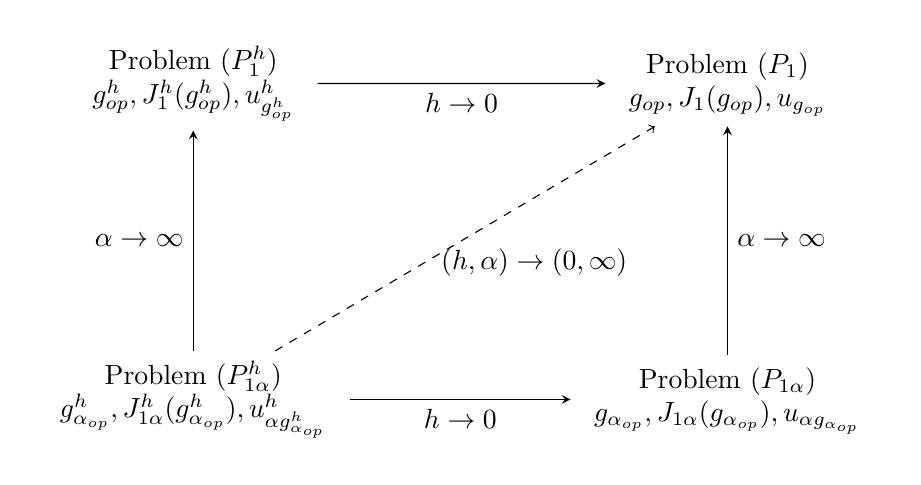
\begin{tikzpicture}
  \matrix (m) [matrix of math nodes,row sep=8em,column sep=8em,minimum width=2em]
  {
     \begin{array}{c} \text{Problem } ({P^h_{1}})\\ {g^h_{op}, J^h_{1}(g^h_{op}),  u^h_{ g^h_{op}}} \end{array}& \begin{array}{c} \text{Problem } (P_{1})\\ g_{op}, J_{1}(g_{op}),  u_{g_{op}} \end{array} \\
   \begin{array}{c} \text{Problem } ({P^h_{1\alpha}})\\ {g^h_{\alpha_{op}}, J^h_{1\alpha}(g^h_{\alpha_{op}}),  u^h_{\alpha g^h_{\alpha_{op}}}} \end{array}& \begin{array}{c} \text{Problem } (P_{1\alpha})\\ g_{\alpha_{op}}, J_{1\alpha}(g_{\alpha_{op}}),  u_{\alpha g_{\alpha_{op}}} \end{array}\\};
  \path[-stealth]
      	 (m-2-1) edge node [left] {$\alpha\to \infty$} (m-1-1)
       
        (m-2-2) edge node [right] {$\alpha\to \infty$} (m-1-2)
        
        (m-1-1) edge node [below] {$h\to 0$} (m-1-2)
        
          (m-2-1) edge [dashed,->] node [below] {$\quad \qquad\qquad (h,\alpha)\to (0,\infty)$}(m-1-2)
        
 		(m-2-1) edge node [below] {$h\to 0$} (m-2-2);
 		
 		
            %edge [double] node [below] {$\mathcal{B}_t$} (m-1-2)
  %  (m-2-1.east|-m-2-2) edge node [below] {$\mathcal{B}_T$}
   %         node [above] {$\exists$} (m-2-2)
 %   (m-1-2) edge node [right] {$\mathcal{B}_T$} (m-2-2)
  %          edge [dashed,-] (m-2-1);
\end{tikzpicture}
\end{center}
\end{scriptsize}
\end{Remark}

\section{Boundary Optimization Problem with Variable \boldmath{$q$}}\label{sec4}%párrafo 4

\subsection{Discrete Problem  ${(P^h_2)}$ Associated with $(P_2)$} %4.1

Under the same considerations given in Section \ref{sec3.1} and taking into account Formula~\eqref{J2-J2alpha}, for a given $q \in Q$, we obtain the following quadratic cost function:
        \begin{equation}\label{J2}
        \begin{array}{ll}
        J_2(q)&=\tfrac{x_0 y_0}{2}\Big\{ q^2 x_0^2 \Big(\tfrac{1}{3} +\tfrac{M_2}{x_0^3}\Big)+q x_0 \Big(-\tfrac{5}{12} g x_0^2-  (b-z_d)\Big)  \\[0.5cm]
       &+\tfrac{2}{15} g^2 x_0^4 +  (b-z_d)^2+\tfrac{2}{3} g x_0^2 (b-z_d) \Big\}.
\end{array}       
       \end{equation}

  \noindent Then, the boundary optimal control of problem $(P_2)$, called $q_{op}$, and the associated continuous optimal state
  are given by:
 
      \begin{equation}\label{ec 4.2}
          q_{op}=\frac{\tfrac{5}{12} g x_0^2+ (b-z_d)}{2 x_0 \big(\tfrac{1}{3}+\tfrac{M_2}{x_0^3}\big)},\qquad u_{q_{op}}(x,y) = -\tfrac{1}{2} g\, x^2 + (g\, x_0 - q_{op}) x +b.
       \end{equation}

      
%  Notice that due to  the symmetry of the domain $D$,  the solution $u$ to the system $(S)$ is independent of $y$.
 % Then, applying a numerical scheme of finite difference and working as in~\cite{BoGaTa2020}, we obtain the solution of the discrete 
 % system $(S_h)$. 

Associated with $(P_2)$, we define  the approximate discrete distributed optimal control problem ${(P^h_2)}$ on the constant heat flux $q$ as

$$ \text{ find }\quad {q^h_{op}}\in \mathbb{R}\quad\text{ such that }\quad
{J^h_2}({q^h_{op}})=\min\limits_{q\in \mathbb{R}} \text{ }{J^h_2}(q)
$$
where the  discrete cost function ${J^h_2}$ is defined by
    
     \[{J^h_2} (q)=  \tfrac{1}{2} \lVert {u^h_q} - z_d \rVert^2_H +  \tfrac{1}{2} M_2 \lVert q \rVert ^2_Q ,\]
     
 \noindent where ${u^h_q}$, given in (\ref{Def uh}), {denotes the discrete approximation for a fixed constant flux $q$}, $h$ is the spatial step, and $z_d$ (the desired state).
 From the definition of the norm over $Q$, it results~that:   
    \[{J^h_2} (q)= \tfrac{1}{2} y_0 \Big\{M_2\,q^2 \,x_0 + \, \sum_{i=1}^n \, \int_{x_i}^{x_{i+1}} [{u^h_q} (x,y) - z_d]^2 \,dx \Big \}\]
     
  \noindent and working algebraically, we get
  \begin{equation}\label{J2h(q)}
    \begin{array}{ll}
  &  {J^h_2}(q)=J_2(q)+\tfrac{x_0 y_0}{2}\Big\{  h \,g \,x_0 \Big[\tfrac{1}{3}q x_0 - \tfrac{5}{24} g x_0^2 - \tfrac{1}{2} (b-z_d)\Big] \\[0.45cm]
    & \qquad + h^2 g \Big[\tfrac{1}{36} x_0^2 g- \tfrac{1}{6}(b-z_d) + \tfrac{1}{12} q \,x_0\Big] + \tfrac{1}{24}  h^3g^2 x_0 + \tfrac{1}{180}  h^4  g^2\Big\}.    
    \end{array}    
  \end{equation}

  %Lema 4.1
\begin{Lemma}\label{Lema J2 J2h}
Given $q\in Q$ and $h>0$, we have
     \begin{equation}\label{ec 4.3} 
        \lvert  {J^h_2}(q) - J_2(q) \rvert  \approx C_7 \, h,
     \end{equation}
     where $C_7 = \tfrac{1}{2}x_0^2\, y_0\,|g| \Big \lvert  \tfrac{1}{3}q x_0-\tfrac{5}{24} gx_0^2-\tfrac{1}{2}(b-z_d) \Big \rvert$ is a constant independent of $h.$
      \end{Lemma}
      
\begin{proof}
It follows immediately from expression \eqref{J2h(q)} for ${J^h_2}$.
   \end{proof}

     
  
 
% \noindent Therefore, we can obtain the following result:
      
%Lema 4.2
\begin{Lemma} Let us consider $h>0.$
    
     \begin{itemize}
      \item[(a)]  The explicit expression for the optimal variable ${q^h_{op}} $ is given by:     
     \begin{equation}\label{qhop}
      {q^h_{op}} =q_{op} - B_1 \,\tfrac{g h}{6} - B_2 \tfrac{g h^2}{24\,x_0} , \qquad 
     \end{equation}
     with   $B_1=B_2=\Big(\tfrac{1}{3} + \tfrac{M_2}{x_0^3}\Big)^{-1}.$
     
     \noindent 
     
      \item[(b)]The following error estimates hold:
     		\begin{equation}\label{qhop-qoo}
     		\lvert {q^h_{op}} - q_{op} \rvert \approx C_8 \, h  ,
     		\end{equation}
     	
     		\begin{equation}\label{J2hqhop-J2qop}
     	    \Big \lvert  {J^h_2}({q^h_{op}}) -  J_{2}(q_{op}) \Big \rvert \approx C_9 \, h,
     	    \end{equation}
     		
        where $C_8$  and $C_9$ are  constants independent of $h$.
     
     \end{itemize}
    \end{Lemma}
    
    
    
  \begin{proof}$ $
  \begin{itemize}
  \item[(a)] From the expression \eqref{J2h(q)} for ${J^h_2}$, we have
\begin{equation*}  
 { \frac{d}{dq} J^h_{2}(q)}= \tfrac{1}{2} x_0^2\, y_0 \Big\{ 2\,x_0 \,q \Big(\tfrac{1}{3} + \tfrac{M_2}{x_0^3} \Big) - \tfrac{5}{12} g \,x_0^2 - (b- z_d)  \\   
     +\tfrac{1}{3} \,g \,x_0\,  h+ \tfrac{1}{12} \,g \,h^2 \Big\}.
     \end{equation*} 
Therefore, $${q^h_{op}}= \frac{\tfrac{5}{12} g x_0^2+ (b-z_d)-\tfrac{1}{12} gh^2-\tfrac{1}{3} g x_0 h}{2 x_0 \big(\tfrac{1}{3}+\tfrac{M_2}{x_0^3}\big)}.$$     
   Taking into account that $q_{op}$ is given by \eqref{ec 4.2}, we obtain Formula \eqref{qhop}.
  \item[(b)]


On one hand, expression \eqref{qhop-qoo} is a direct  consequence of expression (\ref{qhop}) where \mbox{$C_8=\Big| \tfrac{g\,  B_1}{6} \Big|.$}
     
On the other hand, taking into account Formula  \eqref{J2h(q)}  for ${J^h_2}$, it follows that
   \begin{equation}\label{48}
   \begin{array}{ll}
  {J^h_2}({q^h_{op}})- J_2(q_{op}) =J_2({q^h_{op}})-J_2(q_{op})\\[0.45cm]
  + \tfrac{x_0^2y_0}{2} h \,g  \Big[\tfrac{1}{3}{q^h_{op}} x_0 - \tfrac{5}{24} g x_0^2 - \tfrac{1}{2} (b-z_d)\Big] +o(h^2).
  \end{array}
\end{equation}  
  From the definition of $J_2$ given by \eqref{J2} and the explicit expression \eqref{qhop} for ${q^h_{op}}$, we get
  \begin{equation}\label{49}
  \begin{array}{lll}
 &J_2({q^h_{op}})-J_2(q_{op})=\tfrac{x_0^2 y_0}{2}\Big\{ \tfrac{x_0}{B_1}({(q^h_{op})}^2-q_{op}^2)\\[0.45cm]
 & +({q^h_{op}}-q_{op})\Big(-\tfrac{5}{12} g x_0^2-  (b-z_d)\Big)\Big\}\\[0.45cm]
 &=\tfrac{x_0^2 y_0}{2} ({q^h_{op}}-q_{op})\Big( \tfrac{x_0}{B_1}({q^h_{op}}+q_{op}) -\tfrac{5}{12} g x_0^2-  (b-z_d)\Big)\\[0.45cm]
 &=\tfrac{x_0^2 y_0}{12}g h B_1 \Big(-\tfrac{2x_0}{B_1} q_{op} +\tfrac{5}{12} g x_0^2+  b-z_d\Big) +o(h^2).
 \end{array}
  \end{equation}
  
  %  & \qquad + \tfrac{x_0 y_0}{2}\Big\{ h^2 g \Big[\tfrac{1}{36} x_0^2 g- \tfrac{1}{6}(b-z_d) + \tfrac{1}{12} q \,x_0\Big] + \tfrac{1}{24}  h^3g^2 x_0 + \tfrac{1}{180}  h^4  g^2\Big\}.

  
 \noindent Taking into account \eqref{48} and \eqref{49}, we obtain estimate \eqref{J2hqhop-J2qop}   with  $$C_9=\frac{|g| x_0^2 y_0 }{2} \Big\lvert\tfrac{B_1}{6}\Big(-\tfrac{2x_0}{B_1}q_{op}+\tfrac{5 }{12}g x_0^2 +b-z_d \Big)+ \tfrac{1}{3}q_{{op}} x_0 - \tfrac{5}{24} g x_0^2 - \tfrac{1}{2} (b-z_d)\Big\rvert. $$

  \end{itemize}
  \end{proof}

     
  
 % Lema 4.3 
\begin{Lemma} Consider $u_{q_{op}}$, the solution of \eqref{ec 1.1} and \eqref{ec 1.2} for $q= q_{op}$, and ${u^h_{q^h_{op}}}$, 
 the discrete solution given by \eqref{Def uh} for each $h>0$ where $q={q^h_{op}}$ is the optimal variable of the problem ${(P^h_2)}$ given by \eqref{qhop}. Then, we have:
  \begin{equation}  \label{difu-problema2} {\rm (a)} \quad  			      
  				  \lVert {u^h_{q^h_{op}}}- u_{q_{op}}  \rVert _H \approx C_{10}\, h,
  \qquad \qquad
     {\rm (b)}\quad
        \left\lVert \pder[{u^h_{q^h_{op}}}]{x} - \pder[u_{q_{op}}]{x} \right\rVert _H \approx C_{11} \,h,
\end{equation}
 \noindent where $C_{10}$ and $C_{11}$ do not depend on the parameter $h.$
     
\end{Lemma}
   
   
   
\begin{proof}$ $
    \begin{itemize}
      
       \item[(a)] From the definition of $u$ and ${u^h}$ given by \eqref{Def: u y ualpha} and \eqref{Def uh}, respectively, it follows for $i= 1,\ldots, n$ that
  		      \begin{equation}
  		      \begin{array}{ll}
  		       {u^h_{q^h_{op}}}(x,y) - u_{q_{op}}(x,y) =  \tfrac{1}{2} \,g \,x^2-( {q^h_{op}} - q_{op} + g\,i\,h) x + g \,\tfrac{i^2-i}{2}\, h^2 , \quad \\[0.45cm]
  		        =\tfrac{1}{2} \,g \,x^2+h g x\left(\tfrac{B_1}{6}-i \right)+h^2g \left(\tfrac{B_1}{24}\tfrac{x}{x_0}+\tfrac{i(i-1)}{2} \right),\quad \forall x\in [x_i,\,x_{i+1}].
  		        \end{array}
  		        \end{equation}
  		      Then,  
\begin{equation*}
\begin{array}{ll} 
       \lVert {u^h_{q^h_{op}}} - u_{q_{op}}  \rVert _H^2= y_0 \displaystyle\sum\limits_{i=1}^n \displaystyle\int\limits_{x_i}^{x_{i+1}} \Big( {u^h_{q^h_{op}}}(x)-u_{q_{op}}(x)\Big)^2\; dx\\[0.45cm] 
      = x_0\, y_0\, g^2 \Big[\tfrac{1}{108} ( B_1-3)^2 h^2 \,x_0^2+\tfrac{1}{216} h^3\, x_0  (  B_1-3)^2 \\[0.45cm]
      +\frac{1}{8640} h^4\, (72 - 30 B_1 + 5 B_1^2)\Big].
           \end{array}
           \end{equation*}
           
Therefore, we get formula \eqref{difu-problema2} (a) with $C_{10}= \lvert  g (B_1-3)\rvert x_0 \sqrt{\tfrac{x_0 y_0}{108}}$ .
           
           \item [(b)] In the same manner, we get  
            $$\begin{array}{ll}
          &  \left\lVert \pder[{u^h_{q^h_{op}}}]{x} - \pder[u_{q_{op}}]{x}   \right\rVert _H^2 = y_0 \displaystyle \sum\limits_{i=1}^{n} \, \int\limits_{x_i} ^{x_{i+1}} \Big ( g\,x  -({q^h_{op}} - q_{op} ) - h\,g\,i\Big )^2\,dx \\
&=y_0\,g^2\Big[\tfrac{1}{36 }(12 - 6 B_1 + B_1^2) h^2   x_0 +\tfrac{1}{72} (B_1-3) B_1  h^3 +\tfrac{1}{576 }B_1^2  \frac{h^4}{x_0} \Big].
\end{array}$$
  	Then, we get \eqref{difu-problema2} (b) with $$C_{11}=\frac{|g|}{6}\sqrt{x_0 y_0 (12-6B_1+B_1^2)} .$$
 		         
    \end{itemize}
    \end{proof}
       
 \subsection{Discrete Problem  ${(P^h_{2\alpha})}$ Associated with $(P_{2\alpha})$} %4.2
     
    If we suppose that the desired state $z_d$ is  constant in \eqref{J2-J2alpha}, the quadratic cost function  $J_{2\alpha}$ for optimal control problem $(P_{2\alpha})$ is explicitly given by:
 
      \begin{equation}\label{J2alpha-Explicito}
      \begin{array}{ll}
  J_{2\alpha}(q)=\dfrac{x_0 y_0}{2}\Big[ q^2 x_0^2 (D_{1\alpha} +\tfrac{M_2}{x_0^3})+q x_0 \Big(D_{2\alpha} g x_0^2+D_{3\alpha}  (b-z_d) \Big)\\[0.45cm]
   \qquad \qquad +D_{4\alpha} g^2 x_0^4 +D_{5\alpha}  (b-z_d)^2+D_{6\alpha} g x_0^2 (b-z_d) \Big],
  \end{array}
  \end{equation}
  
 \noindent where
\begin{equation}  
  \begin{array}{lll}
  D_{1\alpha}= \tfrac{1}{3}+\tfrac{1}{\alpha x_0}+\tfrac{1}{\alpha^2 x_0^2} ,  \quad & D_{2\alpha}= -\tfrac{5}{12}-\tfrac{5}{3\alpha x_0}-\tfrac{2}{\alpha^2 x_0^2}, \;\\
   D_{3\alpha}=- 1-\tfrac{2}{\alpha x_0},& D_{4\alpha}=\tfrac{2}{15} +\tfrac{2}{3\alpha x_0}+\tfrac{1}{\alpha^2 x_0^2} ,\\
    D_{5\alpha}=1,   & D_{6\alpha}=\tfrac{2}{3}+\tfrac{2}{\alpha x_0} .
  \end{array}
  \end{equation}
 
  
 \noindent Then, the continuous boundary optimization control, called $q_{\alpha_{op}}$,  and the associated state~are: 
\begin{equation} \label{qalphaop}
\begin{array}{ll}
q_{\alpha_{op}}=-\tfrac{D_{2\alpha} g x_0^2+D_{3\alpha} (b-z_d)}{2 x_0 \left(D_{1\alpha}+\tfrac{M_2}{x_0^3}\right)},\\ \\
 u_{\alpha q_{\alpha_{op}}}(x,y) = -\tfrac{1}{2} g\, x^2 + (g\, x_0 - q_{\alpha_{op}}) x + \tfrac{1}{\alpha} (g\,x_0 - q_{\alpha_{op}}) +b .
 \end{array}
 \end{equation} 
 
 %REmark 4.1
 \begin{Remark} Notice that $J_{2\alpha}(q)\to J_2(q) $ for all $q\in Q$ and $q_{\alpha_{op}}\to q_{op}$ when $\alpha \to \infty$. 
\end{Remark}   
   
     
  
    
       \noindent Define the discrete cost function as:
\begin{equation}    
   {  J^h_{2 \alpha}} (q)=  \tfrac{1}{2} \lVert {u^h_{\alpha q}} - z_d \rVert^2_H +  \tfrac{1}{2} M_2 \lVert q \rVert ^2_Q ,
     \end{equation}
where {$u^h_{\alpha q}$} is the solution of ${(S^h_{\alpha})}$ given in (\ref{ec 2.3}) {when $q$ is fixed}. We set the following discrete optimization problem 
 ${(P^h_{2\alpha})}$ on the constant heat flux $q$ as

$$ \text{find }\quad { q^h_{\alpha_{op}}}\in \mathbb{R}\quad\text{ such that }\quad
{ J^h_{2 \alpha}}({ q^h_{\alpha_{op}}})=\min\limits_{q\in \mathbb{R}} \text{ }{ J^h_{2 \alpha}}({q}).
$$
  
    
    
  
  
  Working algebraically, the cost function ${ J^h_{2 \alpha}}$ can be written explicitly as:
  \begin{equation}\label{J2halpha-Explicito}
  \begin{array}{rl}
&  { J^h_{2 \alpha}}(q)= J_{2\alpha}(q) \\[0.45cm]
  &\quad+ \tfrac{1}{2} x_0\,y_0 \,g \,h \Big \{   \tfrac{ q\,x_0^2}{3}   - \tfrac{5\,g x_0^3}{24}  - \tfrac{(b-z_d)\,x_0}{2} 
    + \tfrac{3 x_0 q}{2\,\alpha} - \tfrac{7 g\,x_0^2}{6\alpha}
     - \tfrac{2(b-z_d)}{\alpha}+ \tfrac{2(q-g\,x_0)}{\alpha^2} \\[0.45cm]
    & \quad + h \Big( \tfrac{x_0^2\, g}{36}-  \tfrac{(b-z_d)}{6} + \tfrac{q \,x_0}{12} + \tfrac{2g\,x_0+q}{6\,\alpha}+\tfrac{g}{\alpha^2}\Big)\\[0.45cm]
    & \quad + h^2\,g \Big( \tfrac{x_0}{24} + \tfrac{1}{6\alpha} \Big) + \tfrac{1}{180} g\, h^3 \Big\}. 
    \end{array}
    \end{equation}
     

  
\begin{Lemma}\label{Lema 4.4} For each $q\in Q$  and $h>0$, we have:
\begin{equation}   \lvert  { J^h_{2 \alpha}}(q) - J_{2\alpha}(q) \rvert  \approx C_{7 \alpha} \, h, 
   \end{equation}
      with $$C_{7 \alpha} = \tfrac{1}{2}x_0^2\, y_0\, \Big \lvert g \,  \Big(  \tfrac{ q\,x_0}{3}   - \tfrac{5\,g x_0^2}{24}  - \tfrac{(b-z_d)}{2}+ \tfrac{3 q}{2\,\alpha} - \tfrac{7 g\,x_0}{6\alpha} - \tfrac{2(b-z_d)}{x_0 \,\alpha}+ \tfrac{2(q-g\,x_0)}{x_0\,\alpha^2}\Big)    \Big \rvert, $$ a constant independent of $h.$      
  
\end{Lemma}
\begin{proof}
It follows immediately from expression \eqref{J2halpha-Explicito}.
\end{proof}



%Lema 4.5
\begin{Lemma} Let us consider $h>0.$
    
     \begin{itemize}
      \item[(a)]  The explicit expression for optimal control ${q^h_{\alpha_{op}}} $ is given by:     
     \begin{equation}\label{qhalphaop}
      { q^h_{\alpha_{op}}} = q_{\alpha_{op},}-B_{1\alpha}\frac{gh}{6}-B_{2\alpha}\frac{g h^2}{24 x_0} 
     \end{equation}
     with   $$\begin{array}{cc}
     B_{1\alpha}=\left(1+\tfrac{9}{2\alpha x_0}+\tfrac{6}{\alpha^2 x_0^2}\right) \left(D_{1\alpha}+\tfrac{M_2}{x_0^3} \right)^{-1},\\[0.45cm]
      B_{2\alpha}=\left(1-\tfrac{2}{\alpha x_0}\right) \left(D_{1\alpha}+\tfrac{M_2}{x_0^3} \right)^{-1}.\end{array}$$
     
     \noindent 
     
      \item[(b)]The following error estimates hold:
     		\begin{equation}\label{qhalphaop-qalphaop}
     		\lvert { q^h_{\alpha_{op}}} - q_{\alpha_{op}} \rvert \approx C_{8\alpha} \, h ,
     		\end{equation}
     		\begin{equation}\label{J2halpha qhalphaop-J2alpha qalphaop}
     	    \Big \lvert  { J^h_{2 \alpha}}({ q^h_{\alpha_{op}}}) -  J_{2\alpha}(q_{\alpha_{op}}) \Big \rvert \approx C_{9\alpha} \, h,
     	    \end{equation}
     		     		
    		
        where $C_{8\alpha}$  and $C_{9\alpha}$  do not depend on $h$.
     
     \end{itemize}
    \end{Lemma}
    \begin{proof} $ $
    
    
    
    \begin{itemize}
    \item[(a)]From the derivative of the control function ${ J^h_{2 \alpha}}$ given by
     \begin{equation*}
  \begin{array}{ll}
  { \frac{d}{dq} J^h_{2 \alpha}}(q)= {\frac{d}{dq}J_{2\alpha}}(q) + \tfrac{1}{2} x_0\,y_0 \,g \,h \Big \{   \tfrac{ x_0^2}{3} 
    + \tfrac{3 x_0 }{2\,\alpha} + \tfrac{2}{\alpha^2}
    + h \Big( \tfrac{x_0}{12} + \tfrac{1}{6\,\alpha} \Big) \Big\}\\[0.45cm] 
   \qquad \quad \ \ =\frac{x_0 y_0}{2} \Big\{2qx_0^2 \Big( D_{1\alpha}+\frac{M_2}{x_0^3}\Big) +x_0 \Big(D_{2\alpha} g x_0^2+ D_{3\alpha} (b-zd) \Big)\\[0.45cm]
   \qquad \qquad \; \; +gh\Big(   \tfrac{ x_0^2}{3} + \tfrac{3 x_0 }{2\,\alpha} + \tfrac{2}{\alpha^2}
    + h \Big( \tfrac{x_0}{12} + \tfrac{1}{6\,\alpha} \Big)\Big)\Big\},
    \end{array}
    \end{equation*}
    it follows that
    
      \begin{equation*}
  \begin{array}{ll}
  { q^h_{\alpha_{op}}}=  \frac{- gh\Big(   \tfrac{ x_0^2}{3} 
    + \tfrac{3 x_0 }{2\,\alpha} + \tfrac{2}{\alpha^2}\Big)-g h^2\Big( \tfrac{x_0}{12} + \tfrac{1}{6\,\alpha} \Big)- x_0 \Big(D_{2\alpha} g x_0^2+ D_{3\alpha} (b-zd) \Big)}{2x_0^2  \Big( D_{1\alpha}+\frac{M_2}{x_0^3}\Big)}.
    \end{array}
    \end{equation*}
%     $${ q^h_{\alpha_{op}}}= \frac{- gh\Big(   \tfrac{ x_0^2}{3} 
%     + \tfrac{3 x_0 }{2\,\alpha} + \tfrac{2}{\alpha^2}\Big)-g h^2\Big( \tfrac{x_0}{12} + \tfrac{1}{6\,\alpha} \Big)- x_0 \Big(D_{2\alpha} g x_0^2+ D_{3\alpha} (b-zd) \Big)}{2x_0^2  \Big( D_{1\alpha}+\frac{M_2}{x_0^3}\Big)}.$$
    Working algebraically, we get formula \eqref{qhalphaop}.
    
    \item[(b)] Estimate  \eqref{qhalphaop-qalphaop} follows straightforwardly from \eqref{qhalphaop} with
    $$C_{8\alpha}=\left\lvert  \frac{g B_{1\alpha}}{6}\right\rvert.$$
    
From formula \eqref{J2halpha-Explicito} we obtain that
    \begin{equation}\label{resta1}
    \begin{array}{ll}
    { J^h_{2 \alpha}}({ q^h_{\alpha_{op}}})-J_{2\alpha}(q_{\alpha_{op}})=    J_{2\alpha}({ q^h_{\alpha_{op}}})-J_{2\alpha}(q_{\alpha_{op}}) \\[0.45cm]
    + \tfrac{1}{2} x_0\,y_0 \,g \,h \Big(   \tfrac{ { q^h_{\alpha_{op}}}\,x_0^2}{3}   - \tfrac{5\,g x_0^3}{24}  - \tfrac{(b-z_d)\,x_0}{2} 
    + \tfrac{3 x_0 { q^h_{\alpha_{op}}}}{2\,\alpha}\\[0.45cm]
    - \tfrac{7 g\,x_0^2}{6\alpha} - \tfrac{2(b-z_d)}{\alpha}+ \tfrac{2({ q^h_{\alpha_{op}}}-g\,x_0)}{\alpha^2}\Big)+o(h^2).
    \end{array}
    \end{equation}
Moreover, taking into account the explicit expression for ${J^h_{2\alpha}}$ given by  \eqref{J2halpha-Explicito} and \mbox{Formula~\eqref{qhalphaop}}, it follows that
\begin{equation}\label{resta2}
    \begin{array}{ll}
  {  J^h_{2\alpha}( q^h_{\alpha_{op}}})-J_{2\alpha}(q_{\alpha_{op}})= \frac{x_0^2 y_0}{2}\big({ q^h_{\alpha_{op}}}-q_{\alpha_{op}}\big) \Big[\big({ q^h_{\alpha_{op}}}+q_{\alpha_{op}}\big)x_0  \left(D_{1\alpha}+\tfrac{M_2}{x_0^3} \right)\\
    + D_{2\alpha}g x_0^2+D_{3\alpha}(b-z_d) \Big]\\
=-\frac{x_0^2 y_0}{12}  g B_{1\alpha}  \left(2q_1 x_0 \left(D_{1\alpha}+\frac{M_2}{x_0^3}\right)+D_{2\alpha} g x_0^2+D_{3\alpha} (b-z_d)\right)+o(h^2).
    \end{array}
\end{equation}    
    Combining \eqref{resta1} and \eqref{resta2} we get estimate \eqref{J2halpha qhalphaop-J2alpha qalphaop} with 
    \begin{equation*}
      \begin{array}{ll}
     C_{9\alpha}&=\frac{x_0^2 y_0}{2} |g| \,\Big| -\frac{B_{1\alpha}}{6}\Big(2 q_{\alpha_{op}} x_0 \Big(  D_{1\alpha}+\frac{M_2}{x_0^3}\Big)+D_{2\alpha}gx_0^2+D_{3\alpha}(b-z_d) \Big)\\
     \\
    & +  \frac{ q_{\alpha_{op}}\,x_0}{3}   - \frac{5\,g x_0^2}{24}  - \frac{(b-z_d)}{2} 
     + \frac{3  q_{\alpha_{op}}}{2\,\alpha} - \frac{7 g\,x_0}{6\alpha} - \frac{2(b-z_d)}{\alpha x_0}+ \frac{2(q_{\alpha_{op}}-g\,x_0)}{\alpha^2 x_0}\Big|.
     \end{array}
    \end{equation*}

%     $$\begin{array}{ll}
%     C_{9\alpha}&=\frac{x_0^2 y_0}{2} |g| \,\Big| -\tfrac{B_{1\alpha}}{6}\Big(2 q_{\alpha_{op}} x_0 \Big(  D_{1\alpha}+\tfrac{M_2}{x_0^3}\Big)+D_{2\alpha}gx_0^2+D_{3\alpha}(b-z_d) \Big)\\
%     \\
%    & +  \tfrac{ q_{\alpha_{op}}\,x_0}{3}   - \tfrac{5\,g x_0^2}{24}  - \tfrac{(b-z_d)}{2} 
%     + \tfrac{3  q_{\alpha_{op}}}{2\,\alpha} - \tfrac{7 g\,x_0}{6\alpha} - \tfrac{2(b-z_d)}{\alpha x_0}+ \tfrac{2(q_{\alpha_{op}}-g\,x_0)}{\alpha^2 x_0}
%    \Big|.
%     \end{array}$$
    \end{itemize}
    \end{proof}


%Lema 4.6   
\begin{Lemma} Let us consider $u_{q_{\alpha_{op}}}$ the solution of \eqref{ec 1.1} and \eqref{ec 1.3} for $q= q_{\alpha_{op}}$ and ${u^h_{\alpha q^h_{\alpha_{op}}}}$ the discrete solution  given in (\ref{ec 2.3}) for  $h>0$ and $q={ q^h_{\alpha_{op}}}$. Then, we have:
						
	 \begin{equation}\begin{array}{ll} \label{difu-problema2alpha} {\rm (a)} \quad  			      
  				  \lVert {u^h_{\alpha q^h_{\alpha_{op}}}} - u_{\alpha q_{\alpha_{op}}}  \rVert _H \approx C_{10\,\alpha}\, h,
  \qquad \qquad \\
  \\
     {\rm (b)}\quad
        \left\lVert \pder[{u^h_{\alpha q^h_{\alpha_{op}}}}]{x} - \pder[u_{\alpha q_{\alpha_{op}}}]{x} \right\rVert _H \approx C_{11\, \alpha} \,h,
        \end{array}
\end{equation}
   \end{Lemma}
   
   \begin{proof} Similarly to what was done in Lemma \ref{Lema 4.4}, we obtain
   $$\begin{array}{ll}
   C_{10\, \alpha}=|g|x_0\\
    \sqrt{\tfrac{x_0 y_0}{108}} \sqrt{B_{1\alpha}^2 \left( \tfrac{3}{\alpha^2 x_0^2}+\tfrac{3}{\alpha x_0}+1\right)+9\left(\tfrac{12}{\alpha^2 x_0^2}+\tfrac{6}{\alpha x_0}+1 \right)-3B_{1\alpha}\left( \tfrac{12}{\alpha^2 x_0^2}+\tfrac{9}{\alpha x_0}+2\right)}\end{array}$$
   
   
      $$C_{11\, \alpha}=\frac{|g|}{6} \sqrt{ x_0 y_0 (12-6B_{1\alpha}+B_{1\alpha}^2)}.$$
   \end{proof}
   
%Remark 4.2   
\begin{Remark}
The constants verify that \mbox{$C_{i\alpha}\to C_i$}, when $ \alpha\to\infty, $ for each $ i=7,\dots,11.$
\end{Remark}

%Remark 4.3
\begin{Remark}
The double convergence when $(h,\alpha)\to (0,+\infty)$ of the optimal control of problem ${(P^h_{2\alpha})}$ holds. The relationship among optimal control  problems  $(P_{2})$, $(P_{2\alpha})$, ${(P^h_2)}$ and ${(P^h_{2\alpha})}$ is given by the following diagram:
\begin{scriptsize}
\begin{center}
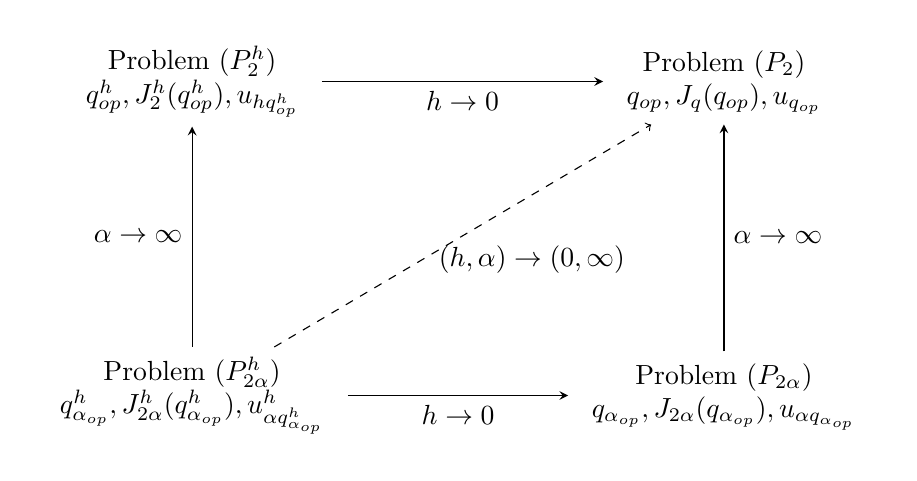
\begin{tikzpicture}
  \matrix (m) [matrix of math nodes,row sep=8em,column sep=8em,minimum width=2em]
  {
     \begin{array}{c} \text{Problem } {(P^h_2)}\\ {q^h_{op}}, {J^h_2}({q^h_{op}}),  u_{h {q^h_{op}}} \end{array}& \begin{array}{c} \text{Problem } (P_{2})\\ q_{op}, J_{q}(q_{op}),  u_{q_{op}} \end{array} \\
   \begin{array}{c} \text{Problem } {(P^h_{2\alpha})}\\ { q^h_{\alpha_{op}}}, { J^h_{2 \alpha}}({ q^h_{\alpha_{op}}}),  {u^h_{\alpha q^h_{\alpha_{op}}}} \end{array}& \begin{array}{c} \text{Problem } (P_{2\alpha})\\ q_{\alpha_{op}}, J_{2\alpha}(q_{\alpha_{op}}),  u_{\alpha q_{\alpha_{op}}} \end{array}\\};
  \path[-stealth]
      	 (m-2-1) edge node [left] {$\alpha\to \infty$} (m-1-1)
       
        (m-2-2) edge node [right] {$\alpha\to \infty$} (m-1-2)
        
        (m-1-1) edge node [below] {$h\to 0$} (m-1-2)
        
          (m-2-1) edge [dashed,->] node [below] {$\quad \qquad\qquad (h,\alpha)\to (0,\infty)$}(m-1-2)
        
 		(m-2-1) edge node [below] {$h\to 0$} (m-2-2);
 		
 		
            %edge [double] node [below] {$\mathcal{B}_t$} (m-1-2)
  %  (m-2-1.east|-m-2-2) edge node [below] {$\mathcal{B}_T$}
   %         node [above] {$\exists$} (m-2-2)
 %   (m-1-2) edge node [right] {$\mathcal{B}_T$} (m-2-2)
  %          edge [dashed,-] (m-2-1);
\end{tikzpicture}
\end{center}
\end{scriptsize}


\end{Remark}

 \vspace{.2cm}
% %   \section{RESULTADOS NUM\'ERICOS}
% %    
% %    En esta secci\'on, se obtienen algunos resultados num\'ericos para los problemas de control \'optimo 
% %    de frontera planteados en (\ref{ec 8} y \ref{ec 9}) y para los sistemas $(S)$ y $(S_\alpha)$ definidos en 
% %    (\ref{ec 1},\ref{ec 2}) y (\ref{ec 1},\ref{ec 3}).
% % 
% %    Se consideran los siguientes datos: $\Omega = [0,1]^2$, $b=30\, \text{\textcelsius} $, $q=12\, \text{\textcelsius} /m$.
% %    Adem\'as, $ g=10 \,\text{\textcelsius}/ m^2$, $z_d= 40 \,\text{\textcelsius}$ el estado deseado y $M=1$. 
% %    El coeficiente de transferencia de calor convectivo $\alpha=1000$ y para el mallado se suponen $h= 1/n$ para $n$ entre $5$ y $30$.
% % 
% %  
% %      Entonces, en la Figura 1 se aprecia el comportamiento de la familia de controles \'optimos discretos  $\{q_{op_h}\}$
% %      cuando el par\'ametro $h= 1/n$ toma distintos valores para $n$ entre $5$ y $30$. Puede verse que la familia 
% %      converge a $q_{op}$ cuando $h \to 0$ que es la soluci\'on del problema de control \'optimo de borde continuo $(P)$
% %      definido en (\ref{ec 8}) como se demostr\'o en la Secci\'on 2. Se nota que esta convergencia es en forma creciente.
% % 
% %      En la Figura 2, se observa la familia de soluciones discretas $\{u_{h\,q_{op_h}}\}_h$, donde el estado $u_{h\,q_{op_h}}$ 
% %      es la soluci\'on del sistema discreto $(S_h)$ definido en  (\ref{ec 1},\ref{ec 3}) asociado al control \'optimo  $q_{op_h}$,
% %      para los distintos valores del par\'ametro $h$ utilizados en la confecci\'on de la figura anterior. Se tiene
% %      nuevamente convergencia de $\{u_{h\,q_{op_h}}\}_h$ a la soluci\'on exacta $u_{op}$ del sistema (\ref{ec 1},\ref{ec 2})
% %      para  $q= q_{op}$ como se vio en el Lema $4 b$. En este caso, la convergencia se da en forma decreciente, es decir que 
% %      $u_{h\,q_{op_h}} \geq u_{op} \qquad \forall \quad h > 0.$
% %      
% %    Adem\'as, en la Figura 3 se observa un comportamiento an\'alogo al descripto en la Figura 1
% %    la familia de controles \'optimos de borde discretos  $\{q_{op_{h\, \alpha}}\}$, definida en (\ref{ec 20}). Es decir, 
% %    que esta familia converge como se ve en el Lema $7 $ y en forma decreciente al control \'optimo continuo $q_{op}$ establecido en (\ref{ec 9}). 
% %    
% %     En la Figura 4, la familia de soluciones discretas $\{u_{h\,q_{op_{h\,\alpha}}}\}_h$  del sistema discreto $(S_{h \,\alpha})$
% %     definido en (\ref{ec 1},\ref{ec 3}), para los distintos valores del par\'ametro $h$ utilizados en la confecci\'on de las figuras anteriores.
% %     Se tiene nuevamente convergencia de $\{u_{h\,q_{op_{h\,\alpha}}}\}_h$ a la soluci\'on exacta $\{u_{op_{\alpha}}\}$ 
% %     del sistema (\ref{ec 1},\ref{ec 2}) como se mostr\'o en el Lema $8 b$. En este caso, la convergencia se da en forma decreciente, es decir que 
% % $ u_{h\,q_{op_{h\,\alpha}}} \geq u_{op_{\alpha}} \qquad \forall \quad h > 0.$
% % 

\section{Boundary Optimization Problem with Variable \boldmath{$b$}}\label{sec5}%párrafo 5

\subsection{Discrete Problem  ${(P^h_{3})}$ Associated with $(P_3)$} %5.1
In this section we consider the boundary optimal control problem  $(P_3)$ given by \eqref{PControlJ3}. 
Taking into account expression \eqref{J3-J3alpha}, for a given constant $b$, we get
    
    \begin{equation}\label{J3-explicito}
    \begin{array}{ll}
     J_3(b)=\tfrac{x_0\,y_0}{2}\Big\{ b^2 \Big(1+ \tfrac{M_3}{x_0} \Big) + b   \Big( \tfrac{2\,g\,x_0^2 }{3}- q\,x_0 - 2\,z_d \Big) \\[0.45cm]
     \hspace{1.4cm}+\Big [\tfrac{2g^2 x_0^4}{15} -\tfrac{5 g q x_0^3}{12} + \tfrac{x_0^2}{3} (q^2-2 g z_d) + z_d(z_d + q x_0) \Big]\Big\}.
     \end{array} 
    \end{equation}

    \noindent Then, the boundary optimal variable of problem $(P_3)$, called $b_{op}$, and the associated continuous optimal state, are given respectively by:
    
    \begin{equation}\label{bop-ubop}
     b_{op}= \frac{-\tfrac{g x_0^2}{3} + \tfrac{q x_0}{2} + z_d}{1+ \tfrac{M}{x_0}}, \qquad 
     u_{b_{op}}=  -\tfrac{1}{2} g\, x^2 + (g\, x_0 - q) x +b_{op}.
    \end{equation}


We define the discrete optimal control problem ${(P^h_{3})}$ on the constant temperature $b$ as

$$ \text{ find }\quad {b^h_{op}}\in \mathbb{R}\quad\text{ such that }\quad
{J^h_{3}}({b^h_{op}})=\min\limits_{b\in \mathbb{R}} \text{ }{J^h_{3}}(b)
$$
where the discrete cost function  ${J^h_{3}}(b)$ is defined as:
    
     \[{J^h_{3}} (b)=  \tfrac{1}{2} \lVert {u^h_b} - z_d \rVert^2_H +  \tfrac{1}{2} M_3 \lVert b \rVert ^2_B, \]
     
 \noindent where ${u^h_b}$ is given in (\ref{Def uh}) {for a fixed constant $b$}, $h$ is the spatial step, and $z_d$ (the desired state) is constant.
 
 
 
Notice that the cost function ${J^h_{3}}$ can be explicitly written as:
   \begin{equation}\label{J3h-explicito}
   \begin{array}{ll}
{J^h_{3}} (b)= J_3(b) +\tfrac{x_0 y_0 g}{2} \Big\{ - b h  \Big( \tfrac{x_0}{2} + \tfrac{h}{6}  \Big) +h  x_0 \big(\tfrac{1}{3} q x_0-\tfrac{5}{24} g x_0^2+\tfrac{z_d}{2} \big)\\[0.45cm]
\hspace{1.45cm}+\tfrac{1}{6} h^2 \Big(\tfrac{q x_0}{2}+\tfrac{1}{6} g  x_0^2+z_d \Big) +\tfrac{1}{24} g h^3 x_0+\tfrac{1}{180}g h^4\Big\}.
\end{array}
\end{equation}

%Lema 5.1
\begin{Lemma}\label{Lema J3 J3h}
Let  $b \in R$ and $h>0$; we have:
    \begin{equation}\label{ec 5.3} 
        \lvert  {J^h_{3}}(b) - J_3(b) \rvert  \approx C_{12} \, h, 
     \end{equation}
     where  $$C_{12} = \tfrac{1}{2}x_0^2\, y_0\,| g| \Big \lvert  -\tfrac{b}{2} + \tfrac{q x_0}{3} -\tfrac{5 g x_0^2}{24} + \tfrac{z_d}{2} \Big \rvert,$$ 
   does not depend on $h.$
      
      \end{Lemma}
\begin{proof}
It follows from expression \eqref{J3h-explicito} for ${J^h_{3}}$.
\end{proof}    \noindent

%Lema 5.2
\begin{Lemma} Let us consider $h > 0$.
    
     \begin{itemize}
      \item[(a)]  The explicit expression for the optimal variable ${b^h_{op}} $ is given by:     
     \begin{equation}\label{bhop}
      {b^h_{op}} =b_{op} + E_1 g x_0 \,h \Big(1+ \tfrac{h}{3 x_0}\Big), \qquad E_1 = \frac{1}{4 \Big(1+ \tfrac{M_3}{x_0} \Big)  }.
     \end{equation}
     
     \noindent 
     
      \item[(b)] The following error estimates hold:
  
     		\begin{equation}\label{bhop-bop}  
     				      \lvert {b^h_{op}} - b_{op} \rvert \approx C_{13} \, h ,
     				      \end{equation}\label{J3hbop-J3bop}
     				      \begin{equation}     		\quad 		     \Big \lvert  {J^h_{3}}({b^h_{op}}) -  J_3(b_{op}) \Big \rvert \approx C_{14} \, h,
     				      \end{equation}
    		
        where $C_{13}$  and $C_{14}$ do not depend on $h$.
     
     \end{itemize}
    
  \end{Lemma}
\begin{proof} $ $


\begin{itemize}
\item[(a)] According to \eqref{J3h-explicito} we have

  \begin{equation}\label{J3h-derivada}
{ \frac{d}{db}J^h_{3}} (b)= \frac{d}{db} J_3(b) -\tfrac{x_0 y_0 }{2} g  b h  \Big( \tfrac{x_0}{2} + \tfrac{h}{6}  \Big) .
\end{equation}
Then, formula \eqref{bhop} for ${b^h_{op}}$ follows immediately.

\item[(b)] Estimate \eqref{bhop-bop}  is a direct consequence of \eqref{bhop} with $C_{13}=|E_1 g x_0|$. 

Moreover, taking into account Formulas \eqref{J3-explicito} and \eqref{J3h-explicito} for $J_3$ and ${J^h_{3}}$ and Formulas \eqref{bop-ubop} and \eqref{bhop} for $b_{op}$ and ${b^h_{op}}$, respectively, it follows that
$$\begin{array}{l}
{J^h_{3}} ({b^h_{op}})- J_3(b_{op})\\[0.45cm]
=J_{3} ({b^h_{op}})- J_3(b_{op}) +\tfrac{x_0^2 y_0 g}{2} \Big\{ - \tfrac{{b^h_{op}}}{2} + \tfrac{1}{3} q x_0-\tfrac{5}{24} g x_0^2+\tfrac{z_d}{2} \Big\} h+ o(h^2).
\end{array}
$$
In addition, the expression  $J_{3} ({b^h_{op}})- J_3(b_{op})$ can be rewritten as
$$
J_{3} ({b^h_{op}})- J_3(b_{op})=\tfrac{x_0^2 y_0 g }{2} E_1   \Big( 2b_{op} \Big(1+ \tfrac{M_3}{x_0} \Big)+\tfrac{2}{3} g x_0^2-q x_0-2 z_d\Big)h+o(h^2).
$$
Therefore, it follows that estimate \eqref{J3hbop-J3bop} is given by  
 \[ C_{14}=  \tfrac{x_0^2  y_0 g}{2} \Big\lvert E_1  \Big( 2b_{op} \Big(1+ \tfrac{M_3}{x_0} \Big)+\tfrac{2}{3} g x_0^2-q x_0-2 z_d\Big)-\tfrac{b_{op}}{2} + \tfrac{q x_0}{3} - \tfrac{5 g x_0^2}{24}+ \tfrac{z_d}{2}\Big \rvert  \textbf{.}\]
\end{itemize}
\end{proof}
            

%Lema 5.3   
\begin{Lemma} Let us consider $u_{b_{op}}$, the solution of \eqref{ec 1.1}, \eqref{ec 1.3} for $b= b_{op}$, and
		${ u^h_{b^h_{op}}}$, the discrete solution  given in (\ref{ec 2.3}) for  $h>0$ and $b={b^h_{op}}.$ Then, we have:
						
	 \begin{equation}  \label{difu-problema3} {\rm (a)} \quad  			      
  				  \lVert {u^h_{b^h_{op}}} - u_{b_{op}}  \rVert _H \approx C_{15}\, h,
  \quad \quad
     {\rm (b)}\quad
        \left\lVert \pder[{u^h_{b^h_{op}}}]{x} - \pder[u_{b_{op}}]{x} \right\rVert _H \approx C_{16} \,h,
\end{equation}
where $C_{15}$ and $C_{16}$ are constants that do not depend on $h$.
   \end{Lemma}   
    
 \begin{proof}
 Working algebraically, we obtain 
$$  \lVert {u^h_{b^h_{op}}} - u_{b_{op}}  \rVert^2 _H=\tfrac{x_0^3  y_0 g^2}{2} \Big(2E_1^2-E_1+\tfrac{1}{6} \Big) h^2+o(h^3). $$
Then, we obtain estimate $\rm (a)$ with
 $$C_{15}=x_0  |g| \sqrt{\tfrac{x_0 y_0}{2}}\sqrt{2E_1^2-E_1+\tfrac{1}{6} }.$$
 In a similar manner, we get that estimate $\rm{b})$ holds with
 $$C_{16}=|g|\sqrt{\tfrac{x_0 y_0}{2}}.$$
 \end{proof}
 
   \subsection{Discrete Problem  ${(P^h_{3\alpha})}$ Associated with $(P_{3\alpha})$} %5.2
  
  
   From~\cite{BoGaTa2020}, we know that  the continuous quadratic  functional cost in \eqref{J1-J1alpha} for the optimization problem  $(P_{3\alpha})$  is explicitly given by: 
      \begin{equation}\label{J3alpha-explicito}
          J_{3\alpha}(b)= J_3(b) +\tfrac{x_0 y_0}{2}\Big\{ \tfrac{1}{3\alpha}  (q - g x_0) (-6b + 3 q x_0 - 2 g x_0^2 + 6 z_d) +  \tfrac{1}{\alpha^2} (  q- g x_0)^2 \Big\}
      \end{equation}
      where $J_3$ is defined by \eqref{J3-explicito}.
      Moreover, the continuous optimal boundary control $b_{\alpha_{op}}$ is given by
\begin{equation}\label{balphaop}
          b_{\alpha_{op}} =b_{op}-  \frac{ g x_0-q}{\alpha (1+ \tfrac{M_3}{x_0})} .
     \end{equation}
\noindent The continuous associated state is established by: 
     \begin{equation}\label{ualpha-balphaop}
\qquad u_{b_{\alpha_{op}}}(x,y) = -\tfrac{1}{2} g\, x^2 + (g\, x_0 - q) x + \tfrac{1}{\alpha} (g\,x_0 - q) +b_{\alpha_{op}} .
       \end{equation}
       
       
     
\vspace{.2cm}
    
\noindent Define the discrete cost function as:
\begin{equation}    
    { J^h_{3\alpha}} (b)=  \tfrac{1}{2} \lVert {u^h_{\alpha b}} - z_d \rVert^2_H +  \tfrac{1}{2} M_3 \lVert b \rVert ^2_B 
     \end{equation}
where ${u^h_{\alpha b}}$ is the solution of ${ (S^h_{\alpha })}$ given in (\ref{ec 2.3}) {for a fixed $b$}.  We set the following discrete optimization problem ${(P^h_{3\alpha})}$ as

$$ \text{find }\quad {b^h_{\alpha_{op}}}\in \mathbb{R}\quad\text{ such that }\quad
{J^h_{3\alpha}}({b^h_{\alpha_{op}}})=\min\limits_{b\in \mathbb{R}} \text{ }{J^h_{3\alpha}}(b).
$$

Working algebraically leads us to write ${J^h_{3\alpha}}$ as follows:
  \begin{equation}\label{J3halpha-Explicito}
  \begin{array}{ll}
 { J^h_{3\alpha}}(b)= J_{3\alpha}(b) + \tfrac{1}{2} x_0\,y_0 \,g \,h \Big \{- b \Big(  \tfrac{x_0}{2} + \tfrac{2}{\alpha}  + \tfrac{h}{6}\Big)
  + g \Big( \tfrac{-5 x_0^3}{24} -  \tfrac{7 x_0^2}{6 \alpha} -  \tfrac{2 x_0}{\alpha^2} \Big)\\[0.45cm]
  + q \Big(  \tfrac{x_0^2}{3} +  \tfrac{3 x_0}{2 \alpha} +  \tfrac{2}{\alpha^2}\Big) + z_d \Big(  \tfrac{x_0}{2} +  \tfrac{2}{\alpha}\Big) \\[0.45cm]
  + h \Big[ g \Big(  \tfrac{x_0^2}{36} +  \tfrac{x_0}{3 \alpha} +  \tfrac{1}{\alpha^2}\Big) + q \Big(  \tfrac{x_0}{12} + \tfrac{1}{6 \alpha}\Big) + \tfrac{z_d}{6} \Big]
 + h^2 g \Big(  \tfrac{x_0}{24} +  \tfrac{1}{6 \alpha}\Big) + h^3 \tfrac{g}{180} \Big\}.
 \end{array}
 \end{equation}
        
  \vspace{.4cm}
%Lema 5.4

  \begin{Lemma} For $b\in B$ and $h>0$, we have
\begin{equation}    \label{J3halpha-J3alpha}
 \lvert  { J^h_{3\alpha}}(b) - J_{3\alpha}(b) \rvert  \approx C_{12\alpha} \, h ,
\end{equation}
with $$C_{12\alpha}=\tfrac{x_0\,y_0}{2}  |g|  \Big\lvert- b \Big(  \tfrac{x_0}{2} + \tfrac{2}{\alpha}  + \tfrac{h}{6}\Big)
  + g \Big( \tfrac{-5 x_0^3}{24} -  \tfrac{7 x_0^2}{6 \alpha} -  \tfrac{2 x_0}{\alpha^2} \Big)
  + q \Big(  \tfrac{x_0^2}{3} +  \tfrac{3 x_0}{2 \alpha} +  \tfrac{2}{\alpha^2}\Big) + z_d \Big(  \tfrac{x_0}{2} +  \tfrac{2}{\alpha}\Big)\Big\rvert.$$
  \end{Lemma}
  \begin{proof}
  It arises immediately from \eqref{J3halpha-Explicito}.
  \end{proof}
  
%Lema5.5
\begin{Lemma} Let us consider $h > 0$.
    
     \begin{itemize}
      \item[(a)]  The explicit expression for optimal control ${b^h_{\alpha_{op}}} $ is given by:     
     \begin{equation}\label{bhalphaop}
      {b^h_{\alpha_{op}}} =b_{\alpha_{op}} + E_1 g x_0 \,h \Big(1+\tfrac{4}{\alpha x_0}+ \tfrac{h}{3 x_0}\Big),
     \end{equation}
     where $E_1$ is given in \eqref{bhop}.
     \noindent 
     
      \item[(b)] The following error estimates hold:
  
     		\begin{equation}\label{bhalphaop-balphaop}  
     				      \lvert {b^h_{\alpha_{op}}} - b_{\alpha_{op}} \rvert \approx C_{13\alpha} \, h ,
     				      \end{equation}\label{J3halphabhalphaop-J3alphabalphaop}
     				      \begin{equation}     		\quad 		     \Big \lvert { J^h_{3\alpha}}({b^h_{\alpha_{op}}}) -  J_{3\alpha}(b_{\alpha_{op}}) \Big \rvert \approx C_{14\alpha} \, h,
     				      \end{equation}
    		
        where $C_{13\alpha}$  and $C_{14\alpha}$ do not depend on $h$.
     
     \end{itemize}
    
  \end{Lemma}
\begin{proof} $ $
\begin{itemize}
\item[(a)] It follows from expression ${J^h_{3\alpha}}$ given by \eqref{J3halpha-Explicito}.

\item[(b)] The estimate in \eqref{bhalphaop-balphaop} is obtained immediately from item $\rm{a)}$ with $$C_{13\alpha}=|E_1| |g| x_0  \Big\lvert 1+\tfrac{4}{\alpha x_0}\Big\rvert.$$


Taking into account \eqref{J3halpha-Explicito} and \eqref{J3alpha-explicito} yields 
$${J^h_{3\alpha}}({b^h_{\alpha_{op}}})-J_{3\alpha}(b_{\alpha_{op}})=J_{3\alpha}({b^h_{\alpha_{op}}})-J_{3\alpha}(b_{\alpha_{op}})+F_{1\alpha}h+o(h^2).$$
with $$F_{1\alpha}=\tfrac{1}{2} x_0^2\,y_0 \,g\Big(- (b_{\alpha_{op}}-z_d) \Big(  \tfrac{1}{2} + \tfrac{2}{\alpha x_0}  \Big)
  + g x_0^2 \Big( \tfrac{-5 }{24} -  \tfrac{7 }{6 \alpha x_0} -  \tfrac{2 }{\alpha^2 x_0^2} \Big)
  + q x_0\Big(  \tfrac{1}{3} +  \tfrac{3 }{2 \alpha x_0} +  \tfrac{2}{\alpha^2 x_0^2}\Big) \Big).$$

In addition, from  the definition of ${ J^h_{3\alpha}}$ and ${b^h_{\alpha_{op}}}$, we have
$${ J^h_{3\alpha}}({b^h_{\alpha_{op}}})-J_{3\alpha}(b_{\alpha_{op}})=J_3({b^h_{\alpha_{op}}})-J_3(b_{\alpha_{op}})+F_{2\alpha}h+o(h^2)$$
with $$ F_{2\alpha}=\tfrac{x_0^2 y_0 g}{\alpha} E_1 (-q+gx_0)\left( 1+\tfrac{4}{\alpha x_0}\right).$$

Finally, according to formula \eqref{J3-explicito} for $J_3$, we get 
$$J_3({b^h_{\alpha_{op}}})-J_3(b_{\alpha_{op}})=F_{3\alpha}h+o(h^2),$$
with  $$F_{3\alpha}=\tfrac{x_0^2 y_0 g }{2} E_1 \Big( 1+\tfrac{4}{\alpha x_0}\Big)  \Big( 2b_{\alpha_{op}} \Big(1+ \tfrac{M_3}{x_0} \Big)+\tfrac{2}{3} g x_0^2-q x_0-2 z_d\Big).$$


Therefore,  estimate \eqref{J3halphabhalphaop-J3alphabalphaop} holds for 
$$
C_{14\alpha}=\Big\lvert F_{1\alpha}+F_{2\alpha}+F_{3\alpha}\Big\rvert. $$
\end{itemize}
\end{proof}


%Lema 5.6   
\begin{Lemma} Let us consider $u_{b_{\alpha_{op}}}$, the solution of \eqref{ec 1.1} and \eqref{ec 1.3} for $b= b_{\alpha_{op}}$, and
		${u^h_{\alpha b^h_{\alpha_{op}}}}$, the discrete solution  given in (\ref{ec 2.3}) for  $h>0$ and $b={b^h_{\alpha_{op}}}.$ Then, we have:
						
	 \begin{equation}  \label{difu-problema3alpha} {\rm (a)} \quad  			      
  				  \lVert {u^h_{\alpha b^h_{\alpha_{op}}}} - u_{\alpha b_{\alpha_{op}}}  \rVert _H \approx C_{15\,\alpha}\, h,
 \quad
     {\rm (b)}\quad
        \left\lVert \pder[{u^h_{\alpha b^h_{\alpha_{op}}}}]{x} - \pder[u_{\alpha b_{\alpha_{op}}}]{x} \right\rVert _H \approx C_{16\, \alpha} \,h,
\end{equation}
   \end{Lemma}
   
   \begin{proof} Similarly to what was done in Lemma \ref{Lema 4.4}, we obtain
   $$\begin{array}{c}
   C_{15\, \alpha}=x_0  |g|  \sqrt{\tfrac{x_0 y_0}{2}} \mathcal{A}, \\[0.45cm]
  \mathcal{A}= \sqrt{E_1^2\left(2+\tfrac{16}{\alpha x_0}+\tfrac{32}{\alpha^2x_0^2} \right)+E_1\left(-1-\tfrac{8}{\alpha x_0}-\tfrac{16}{\alpha^2 x_0^2} \right)+\tfrac{1}{6}+\tfrac{1}{\alpha x_0}+\tfrac{2}{\alpha^2 x_0^2} },\\[0.45cm]
  C_{16\, \alpha}=C_{16}.
   \end{array}$$
   \end{proof}
   %Remark 5.1
\begin{Remark}
The constants obtained in the estimates of the previous lemmas verify that \mbox{$C_{i\alpha}\to C_i$}  when $ \alpha\to\infty$ for $i=12,\cdots,16$.
\end{Remark}

%Remark 5.2
\begin{Remark}
The double convergence when $(h,\alpha)\to (0,+\infty)$ of the optimal control of problem ${(P^h_{3\alpha})}$ holds. The relationship among the optimal control of problems  $(P_{3})$, $(P_{3\alpha})$, ${(P^h_{3})}$ and ${(P^h_{3\alpha})}$  is given by the following diagram:
\begin{scriptsize}
\begin{center}
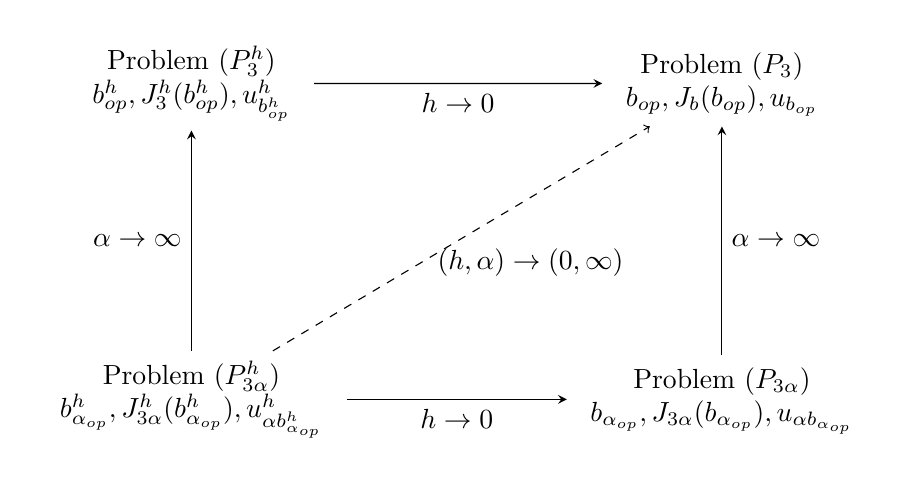
\begin{tikzpicture}
  \matrix (m) [matrix of math nodes,row sep=8em,column sep=8em,minimum width=2em]
  {
     \begin{array}{c} \text{Problem } {(P^h_{3})}\\ {b^h_{op}}, {J^h_{3}}({b^h_{op}}),  {u^h_{b^h_{op}}} \end{array}& \begin{array}{c} \text{Problem } (P_{3})\\ b_{op}, J_{b}(b_{op}),  u_{b_{op}} \end{array} \\
   \begin{array}{c} \text{Problem } {(P^h_{3\alpha})}\\ {b^h_{\alpha_{op}}},{ J^h_{3\alpha}}({b^h_{\alpha_{op}}}),  {u^h_{\alpha b^h_{\alpha_{op}}}}\end{array}& \begin{array}{c} \text{Problem } (P_{3\alpha})\\ b_{\alpha_{op}}, J_{3\alpha}(b_{\alpha_{op}}),  u_{\alpha b_{\alpha_{op}}} \end{array}\\};
  \path[-stealth]
      	 (m-2-1) edge node [left] {$\alpha\to \infty$} (m-1-1)
       
        (m-2-2) edge node [right] {$\alpha\to \infty$} (m-1-2)
        
        (m-1-1) edge node [below] {$h\to 0$} (m-1-2)
        
          (m-2-1) edge [dashed,->] node [below] {$\quad \qquad\qquad (h,\alpha)\to (0,\infty)$}(m-1-2)
        
 		(m-2-1) edge node [below] {$h\to 0$} (m-2-2);
 		
 		
            %edge [double] node [below] {$\mathcal{B}_t$} (m-1-2)
  %  (m-2-1.east|-m-2-2) edge node [below] {$\mathcal{B}_T$}
   %         node [above] {$\exists$} (m-2-2)
 %   (m-1-2) edge node [right] {$\mathcal{B}_T$} (m-2-2)
  %          edge [dashed,-] (m-2-1);
\end{tikzpicture}
\end{center}
\end{scriptsize}

\end{Remark}



\section{Numerical Results}\label{sec6}%3.3
  We carried out some numerical simulations in order to illustrate  the theoretical results obtained in the previous sections for the optimal control problems ${(P^h_{i})}$ and ${(P^h_{i\alpha})}$ for $i=1,2,3$. 
  
  
  Throughout this section we consider the domain $\Omega=[0,1]\times [0,1]$, i.e, $x_0=y_0=1$.



Before analyzing the optimal control problems we illustrate the behavior of the continuous state of the systems $(S)$ and $(S_\alpha)$ and the discrete state of the systems $(S_{h})$ and~$({S^h_\alpha})$.


In Figure \ref{fig1} (a) we plotted the state of system $u$ given by \eqref{Def: u y ualpha} and the approximate  discrete function ${u^h}$ defined by \eqref{Def uh} against the position $x$ for  $h=1/3, 1/5, 1/10$. As we saw in Lemma \ref{Cota u uh} for each fixed $x$, the functions ${u^h}(x)$ increase and get closer to the limit $u(x)$ as $h$ decreases. 
In a similar manner, in Figure \ref{fig1} (b), for $\alpha=50$,  we obtained system $u_\alpha$ given by \eqref{Def: u y ualpha} and the approximate  discrete function ${u^h_\alpha}$ defined by \eqref{ec 2.3} against the position $x$ for  $h=1/3, 1/5, 1/10$.
Notice that as  $h$ decreases, the functions $\lbrace{{u^h_\alpha}\rbrace}$ increase and get closer to the limit $u_\alpha$ as it was proved in Lemma \ref{lema convergencia uhalpha a ualpha}.
\vspace{-3pt}

  \begin{figure}[h]
\centering
\begin{tabular}{cc}
\includegraphics[scale=0.5]{1Graficauuh.png} &
\includegraphics[scale=0.5]{2Graficaualphauhalpha50.png} \\
{\scriptsize (a) $u$ and ${u^h}$ for different values of $h$} &
{\scriptsize (b) $u_\alpha$ and ${u^h_\alpha}$ for different values of $h$ with $\alpha=50$}
\end{tabular}

\caption{State of systems $(S)$, $({S^h})$, $(S_\alpha)$ and $({S^h_\alpha})$ using $q=12$, $b=30$, $z_d=40$ and $g=10$.}
\label{fig1}
\end{figure}

 
  In addition in order to visualize the double convergence of ${u^h_\alpha}\to u$ when \mbox{$(h,\alpha)\to (0,\infty)$,} in Figure \ref{uuhalpha} we plotted $u$ and ${u^h_\alpha}$ for $(h,\alpha)=(1/3,10), (1/5,50)$ and $(1/10,500)$.


 
 \begin{figure}[h!!]
 \centering
 \includegraphics[scale=0.6]{3Graficauuhalpha.png}
\caption{Plot of $u$ and ${u^h_\alpha}$ against $n=1/h$ for different values of $(h,\alpha)$.}\label{uuhalpha}
 \end{figure}
 

 
 
 {Table \ref{tab:L2errors} illustrates that the $L^2$ errors exhibit a linear rate of convergence. 
Indeed, each refinement step in which the mesh size $h$ is divided by two produces an error that is approximately halved, confirming the expected first-order behavior.}
\begin{table}[h!!]
\caption{$L^2$ errors for $u-u^h$ and $u_{\alpha}-u_{\alpha}^h$ for different values of $\alpha$.}
\label{tab:L2errors}
\centering
\begin{tabularx}{\textwidth}{c cccc}
\toprule
\boldmath{$h$} &\boldmath{$\|u-u^h\|_{L^2}$}
& \multicolumn{3}{c}{\boldmath{$\|u_{\alpha}-u_{\alpha}^h\|_{L^2}$}} \\
\midrule
 &  & $\alpha=50$ 
      & $\alpha=100$ 
      & $\alpha=200$ \\
\midrule
0.250000 & 7.675914 × 10\textsuperscript{$-$1}%MDPI: Please use the scientific notation, e.g., "$8 \times 10^{3}$", not "8E3". We corrected them. Please confirm. Same as below.
 & 8.120374 × 10\textsuperscript{$-$1} & 7.897314 × 10\textsuperscript{$-$1} & 7.786397 × 10\textsuperscript{$-$1} \\
\midrule
0.125000 & 3.722243 × 10\textsuperscript{$-$1} & 3.942740 × 10\textsuperscript{$-$1} & 3.832039 × 10\textsuperscript{$-$1} & 3.777023 × 10\textsuperscript{$-$1} \\
\midrule
0.062500 & 1.832549 × 10\textsuperscript{$-$1} & 1.942324 × 10\textsuperscript{$-$1} & 1.887200 × 10\textsuperscript{$-$1} & 1.859813 × 10\textsuperscript{$-$1} \\
\midrule
0.031250 & 9.091783 × 10\textsuperscript{$-$2} & 9.639423 × 10\textsuperscript{$-$2} & 9.364392 × 10\textsuperscript{$-$2} & 9.227771 × 10\textsuperscript{$-$2} \\
\midrule
0.015625 & 4.528211 × 10\textsuperscript{$-$2} & 4.801716 × 10\textsuperscript{$-$2} & 4.664351 × 10\textsuperscript{$-$2} & 4.596121 × 10\textsuperscript{$-$2} \\
\bottomrule
\end{tabularx}

\end{table}


 \subsection{Control Variable $g$}
 
 
   In this subsection we obtain some computational examples for the optimal distributed control problems $(P_1)$, ${(P^h_1)}$, $(P_{1\alpha})$ and ${(P^h_{1\alpha})}$. For each plot, we set $q=12, b=30, z_d=40$ and $M_1=1$.
     
     

    
    
    In Figure \ref{figJ1J1h} we plotted the continuous quadratic cost function $J_1$ given by \eqref{J1-explicito}  and the discrete cost function ${J^h_1}$ obtained in \eqref{J1h-explicito} against $g$ for  $h=1/10$, $1/50$ and $1/100$. Notice that as $h$ decreases, the function ${J^h_1}={J^h_1}(g)$  also decreases to the limit function $J_1=J_1(g)$ in agreement with Lemma \ref{Lema:J1(g)-J1h(g)}. In a similar manner in Figure \ref{FigJ1alphaJ1halpha}, for $\alpha=50$, we obtain the continuous function $J_{1\alpha}$ and the discrete functions ${J^h_{1\alpha}}$ for $h=1/10,1/50$ and $1/100$ observing the convergence of ${J^h_{1\alpha}}\to J_{1\alpha}$ as $h$ decreases to zero.
     Moreover, Figure \ref{figJ1double} shows the double convergence of ${J^h_{1\alpha}}\to J_1$ when $(h,\alpha)\to (0,\infty)$. We illustrate how ${J^h_{1\alpha}}$ gets closer to $J_1$ as the value of $h$ decreases and the value of $\alpha$ increases. 
     
  

%------------------ Primera fila ------------------%
\begin{figure}[h!]
\centering
\includegraphics[scale=0.5]{5GraficaJ1J1h.png}
\caption{Plot of $J_1$ and $J^h_1$ against $g$.}
\label{figJ1J1h}
\end{figure}



\begin{figure}[h!]
\centering
\includegraphics[scale=0.5]{6GraficaJ1alphaJ1halpha50.png}
\caption{Plot of $J_{1\alpha}$ and $J^h_{1\alpha}$ for $\alpha=50$ against $g$.}
\label{FigJ1alphaJ1halpha}
\end{figure}

\begin{figure}[h!]
\centering
\includegraphics[scale=0.5]{7GraficaJ1halphaJ1.png}
\caption{Plot of $J_1$ and $J^h_{1\alpha}$ against $g$.}
\label{figJ1double}
\end{figure}



In Figure \ref{figgop} we plotted the continuous optimal control $g_{op}$  for problem $(P_1)$ given by \eqref{gop}  and optimal control $g_{\alpha_{op}}$ given by \eqref{galphaop} for $\alpha=15, 50, 100$. Notice  that as $\alpha$ increases, $g_{\alpha_{op}}$ decreases  to the limit $g_{op}$. 
In addition, we set different values of $n$ between $n=10$ and $n=100$. Recalling that $h=\tfrac{x_0}{n}=\tfrac{1}{n}$, for each $h$, we obtained the optimal discrete control ${g^h_{op}}$ to problem ${(P^h_1)}$ defined by \eqref{lema:goph} and the optimal discrete control  ${g^h_{\alpha_{op}}}$ to problem ${(P^h_{1\alpha})}$ given by \eqref{galphaop} for $\alpha=15, 50, 100$. For each $\alpha$ fixed, we observe the discrete solution ${g^h_{\alpha_{op}}}\to g_{\alpha_{op}}$ when $h\to 0$, i.e., $n\to\infty$.


\begin{figure}[h!]
\centering
\includegraphics[scale=0.5]{4Graficagop.png}
\caption{Plot of $g_{op}$, $g^h_{op}$, $g_{\alpha_{op}}$ and $g^h_{\alpha_{op}}$ against $n=1/h$.}
\label{figgop}
\end{figure}
%------------------ Primera fila ------------------%




 \subsection{Control Variable $q$}
 
 
   In this subsection we ran some computational examples for the optimal boundary control problems $(P_2)$, ${(P^h_2)}$, $(P_{2\alpha})$ and ${(P^h_{2\alpha})}$. For each plot, we set $g=10, b=50, z_d=40$ and $M_2=1$.
  
    In Figure \ref{figJ2J2h} we plotted the continuous quadratic cost function $J_2$ given by \eqref{J2}  and the discrete cost function ${J^h_2}$ obtained in \eqref{J2h(q)} against $q$ for  $h=1/10$, $1/25$ and $1/50$. Observe that as $h$ decreases, function ${J^h_2}={J^h_2}(q)$  also decreases to the limit function $J_2=J_2(q)$. In a similar way, in Figure \ref{FigJ2alphaJ2halpha}, for $\alpha=100$, we obtained the continuous function $J_{2\alpha}$ and the discrete functions ${ J^h_{2 \alpha}}$ for $h=1/10,1/25$ and $1/50$. The convergences ${J^h_2}\to J_2$ and ${ J^h_{2 \alpha}}\to J_{2\alpha}$ when $h\to 0$ are in agreement with Lemmas \ref{Lema J2 J2h} and \ref{Lema 4.4}, respectively.
    
    \begin{figure}[h!]
\centering
\includegraphics[scale=0.5]{8GraficaJ2J2h.png}
\caption{Plot of $J_2$ and $J^h_2$ against $q$.}
\label{figJ2J2h}
\end{figure}


     \begin{figure}[h!]
     \centering
\includegraphics[scale=0.5]{9GraficaJ2alphaJ2halpha100.png}
\caption{Plot %MDPI: Some content is overlap, please check if this figure should be revise.
 of $J_{2\alpha}$ and {$J^h_{2\alpha}$} for $\alpha=100$ against $q$.}
\label{FigJ2alphaJ2halpha}

\end{figure}



     Moreover, Figure \ref{FigJ2dobleconvergencia}  shows the double convergence of ${ J^h_{2 \alpha}}\to J_2$ when $(h,\alpha)\to (0,\infty)$. We illustrate how ${ J^h_{2 \alpha}}$ gets closer to $J_2$ as the value of $h$ decreases and the value of $\alpha$ increases. 
     
     

     \begin{figure}[h!]
     \centering
\includegraphics[scale=0.5]{91GraficaJ2halphaJ2.png}
\caption{Plot %MDPI: Some content is overlap, please check if this figure should be revise.
 of $J_2$ and {$J^h_{2\alpha}$ against $q$}.}
\label{FigJ2dobleconvergencia}

\end{figure}


In Figure \ref{Figqop} we plotted the continuous optimal control $q_{op}$  for problem $(P_2)$ given by \eqref{ec 4.2} and optimal control $q_{\alpha_{op}}$ given by \eqref{qalphaop} for $\alpha=50,  100, 200$. Notice  that as $\alpha$ increases, $q_{\alpha_{op}}$ decreases  to the limit $q_{op}$. 
In addition, we set different values of $n$ between $n=10$ and $n=100$. Recalling that $h=\tfrac{x_0}{n}=\tfrac{1}{n}$, for each $h$, we obtained the optimal discrete control   ${q^h_{op}}$ to problem ${(P^h_2)}$ defined by \eqref{qhop} and the optimal discrete control  ${ q^h_{\alpha_{op}}}$ to problem ${(P^h_{2\alpha})}$ given by \eqref{qhalphaop} for $\alpha=50, 100, 200$. For each $\alpha$ fixed, we observe the discrete solution ${ q^h_{\alpha_{op}}}\to q_{\alpha_{op}}$ when $h\to 0$, i.e., $n\to\infty$.


     \begin{figure}[h!]
          \centering
\includegraphics[scale=0.5]{8Graficaqop.png}
\caption{Plot %MDPI: Some content is overlap, please check if this figure should be revise.
 of $q_{op}$, {$q^h_{op}$}, $q_{\alpha_{op}}$ and {$q^h_{\alpha_{op}}$ against $n=1/h$}.}
\label{Figqop}

\end{figure}

%------------------ Primera fila ------------------%



     \newpage
 
 \subsection{Control Variable $b$}
 
   In this section we obtain some computational examples for the optimal distributed control problems $(P_3)$, ${(P^h_{3})}$, $(P_{3\alpha})$ and ${(P^h_{3\alpha})}$. For each plot, we set $q=12, g=10, z_d=40$ and $M_3=1$.
     
     

    
    
  


\begin{figure}[H]
     \centering
\includegraphics[scale=0.5]{93GraficaJ3J3h.png}
\caption{Plot of $J_3$ and {$J^h_{3}$ against $b$}.}
\label{FigJ3J3h}
\end{figure}


  In Figure \ref{FigJ3J3h} we plotted the continuous quadratic cost function $J_3$ given by \eqref{J3-explicito} and the discrete cost function ${J^h_{3}}$ obtained in \eqref{J3h-explicito} against $g$ for  $h=1/10$, $1/25$ and $1/100$. Notice that as $h$ decreases, function ${J^h_{3}}={J^h_{3}}(b)$  also decreases to the limit function $J_3=J_3(b)$ in agreement with Lemma \ref{Lema J3 J3h}. In a similar manner, in Figure \ref{FigJ3alphaJ3halpha}, for $\alpha=50$, we obtained the continuous function $J_{3\alpha}$ and the discrete functions ${J^h_{3\alpha}}$ for $h=1/10,1/25$ and $1/100$. Observe the convergence of ${J^h_{3\alpha}}\to J_{3\alpha}$ as $h\to 0$.
     Moreover, Figure \ref{FigJ3dobleconvergencia} shows the double convergence of ${J^h_{3\alpha}}\to J_3$ when $(h,\alpha)\to (0,\infty)$. We illustrate how ${J^h_{3\alpha}}$ gets closer to $J_3$ as the value of $h$ decreases and the value of $\alpha$ increases. 

In Figure \ref{Figbop} we plotted the continuous optimal control $b_{op}$  for problem $(P_3)$ given by \eqref{bop-ubop}  and optimal control $b_{\alpha_{op}}$ given by \eqref{balphaop} for $\alpha=15, 50, 100$. Notice  that as $\alpha$ increases, $b_{\alpha_{op}}$ decreases  to the limit $b_{op}$. 
In addition, we set different values of $n$ between $n=10$ and $n=100$. Recalling that $h=\tfrac{x_0}{n}=\tfrac{1}{n}$, for each $h$, we obtained the optimal discrete control   ${b^h_{op}}$ to problem ${(P^h_{3})}$ defined by \eqref{bhop} and the optimal discrete control  ${b^h_{\alpha_{op}}}$ to problem ${(P^h_{3\alpha})}$ given by \eqref{bhalphaop} for $\alpha=15, 50, 100$. For each $\alpha$ fixed, we observe the discrete solution ${b^h_{\alpha_{op}}}$  decreases to $b_{\alpha_{op}}$ when $h\to 0$.


\begin{figure}[h!]
     \centering
\includegraphics[scale=0.5]{94GraficaJ3alphaJ3halpha50.png}
\caption{Plot of $J_{3\alpha}$ and {$J^h_{3\alpha}$} for $\alpha=100$ {against $b$}.}
\label{FigJ3alphaJ3halpha}
\end{figure}


\begin{figure}[h!]
     \centering
\includegraphics[scale=0.5]{95GraficaJ3halphaJ3.png}
\caption{Plot of $J_3$ and $J_{3\alpha}$ {against $b$}.}
\label{FigJ3dobleconvergencia}
\end{figure}


\newpage

\begin{figure}[H]
     \centering
\includegraphics[scale=0.5]{92Graficabop.png}
\caption{Plot %MDPI: Some content is overlap, please check if this figure should be revise.
 of $b_{op}$, {$b^h_{op}$}, $b_{\alpha_{op}}$ and {$b^h_{\alpha_{op}}$ against $n=1/h$}.}
\label{Figbop}
\end{figure}



%------------------ Primera fila ------------------%



\section{Improvement of the Order of Convergence}\label{sec7}
In this section, we introduce alternative discrete solutions ${\widetilde{u}^h}$ and ${\widetilde{u}^h_\alpha}$ associated with systems $(S)$ and $(S_\alpha)$, respectively, and analyze the order of convergence of ${\widetilde{u}^h}$ to $u$ and of ${\widetilde{u}^h_\alpha}$ to $u_\alpha$ as $h \to 0^+$. The Neumann boundary condition on $\Gamma_2$ is approximated by a three-point backward finite-difference scheme. Moreover, for the discrete solution ${\widetilde{u}^h_\alpha}$, the Robin boundary condition on $\Gamma_1$ is approximated by a three-point forward finite-difference scheme. These higher-order boundary approximations lead to an improved order of accuracy.





We consider the system $(S)$ defined by Equations \eqref{ec 1.1} and \eqref{ec 1.2}. From this system, we define the discrete problem ${(\widetilde{S}^h)}$, where {for a fixed $h>0$}, $ {\widetilde{u}^h_i}$ approximates $u(x_i,y)$, for $i=1,\cdots, n+1$. Notice that from the Dirichlet condition on $\Gamma_1$, it follows immediately that ${\widetilde{u}^h_1} = b$.


For the interior nodes, we employ the classical centered second-order finite-difference approximation given in \eqref{aprox-deriv}, which leads to the discrete system \eqref{aprox-nodo-interior} for ${\widetilde{u}^h_i}$, $i=2,...,n$. 

For the Neumann boundary condition on $\Gamma_2$, we use the three-point backward \mbox{approximation}
\begin{equation}\label{aprox-Neumann-nueva}
\pder[u]{x}(x_{n+1},y)\approx \frac{3u(x_{n+1},y)-4u(x_n,y)+u(x_{n-1},y)}{2h}.
\end{equation}
Thus, the discrete Neumann condition can be written as
\begin{equation}
-2 q h = {
3\widetilde{u}^{h}_{n+1}
-4\widetilde{u}^{h}_{n}
+\widetilde{u}^{h}_{n-1}}.
\end{equation}
In addition, from \eqref{aprox-nodo-interior} for $i=n$, we obtain
\begin{equation}
-gh^2 = {\widetilde{u}^h_{n+1}-2\widetilde{u}^h_n+\widetilde{u}^h_{n-1}.}
\end{equation}
Subtracting the two previous equations, it follows that
\begin{equation}\label{aprox-nueva}
{-\widetilde{u}^h_n+\widetilde{u}^h_{n+1}}=\frac{gh^2}{2}-qh.
\end{equation}
Therefore, the system given by \eqref{aprox-nodo-interior} together with \eqref{aprox-nueva} can be written  as
\begin{equation}\label{sistema-nuevo}
{A w^h=\widetilde{T}^h}
\end{equation}
where $w^h = ({\widetilde{u}^h_i})_{i=2,\ldots,n+1}\in\mathbb{R}^{n}$ is the vector of unknowns, $A$ is the matrix given by \eqref{matrizA} and   ${\widetilde{T}^h}\in \mathbb{R}^n$ is the vector of independent terms:
    \begin{equation}\label{vectorT*}
     {\widetilde{T}^h}= \Big(-g\,h^2 - b, -g h^2, \ldots, -g h^2, -q\,h +\tfrac{gh^2}{2} \Big)^t.
\end{equation}
Notice that system \eqref{sistema-nuevo} differs from \eqref{sistema-tradicional} in the last component of the vector of independent terms.
Solving the linear system gives
\begin{equation}
{\widetilde{u}^h_i}=b+(i-1)h(gx_0-q)-\frac{gh^2}{2}(i-1)^2.
\end{equation}
Taking into account that for $i=1,\cdots, n$
\begin{equation}
\widetilde{m}_i={\frac{\widetilde{u}^h_{i+1}-\widetilde{u}^h_{i}}{x_{i+1}-x_i}}=gx_0-q-(2i-1)\frac{gh}{2},
\end{equation}
and
\begin{equation}
\widetilde{h}_i= {\widetilde{u}^h_i-\widetilde{m}_i x_i}= b+\frac{gh^2}{2} i (i-1),
\end{equation}
the linear approximation is given by ${\widetilde{u}^h}(x,y)=\widetilde{m}_i x+\widetilde{h}_i$, i.e.,

\vspace{-12pt}

\centering %% If there is a figure in wide page, please release command \centering
\begin{equation}\label{uhtilde}
{\widetilde{u}^h}(x,y)=\left(gx_0-q-(2i-1)\frac{gh}{2} \right)x+\frac{gh^2}{2} i (i-1)+b,\qquad x\in [x_i,x_{i+1}], \quad i=1,\cdots,n
\end{equation}




In the following lemma, we give some bounds for the approximate  function ${\widetilde{u}^h}:$

 
  \begin{Lemma} \label{Cota u uh tilde} The following  bounds hold:
    		\[\lVert u-{\widetilde{u}^h} \rVert _H \leq  D_1 h^2, \qquad \text{and}\qquad
\lVert \pder[u]{x}-\pder[{\widetilde{u}^h}]{x} \rVert _H \leq \widetilde{D}_{1}\, h, \]
    		where $D_1=\sqrt{\frac{x_0 y_0 }{120}} g $ 
   and $\widetilde{D}_1=\sqrt{\frac{x_0 y_0}{12}}\; g$.
    
    \end{Lemma}
\begin{proof} 
From the definition of the norm in space $H$ and using the expressions \eqref{Def: u y ualpha} and \eqref{uhtilde} for functions $u$ and ${\widetilde{u}^h}$, respectively, it follows that
\begin{equation}\label{cuenta-intermedia}
\begin{aligned}
\|u-{\widetilde{u}^h}\|_{H}^2
&= \int_0^{y_0} \int_0^{x_0} \big(u(x,y)-{\widetilde{u}^h}(x,y)\big)^2 \, \dee x \, \dee y \\[1ex]
&= y_0 \sum_{i=1}^n \int_{x_i}^{x_{i+1}} E_i^2(x)\, \dee x,
\end{aligned}
\end{equation}
where 
\[
E_i(x) = u(x,y) - {\widetilde{u}^h}(x,y), \quad x \in [x_i, x_{i+1}], \; y \in [0, y_0].
\] 
Note that, within each subinterval, $E_i(x)$ depends only on $x$ and the index $i$, but not on $y$, since both $u$ and ${\widetilde{u}^h}$ are constant along the $y$-direction.  

A direct computation yields
\begin{equation}\label{Ei}
E_i(x) = \frac{g}{2} \Big(-x^2 + (2i-1) h x - h^2 i(i-1) \Big) 
= -\frac{g}{2} (x - i h)(x - (i-1) h).
\end{equation}

Then,
\begin{equation}\label{integralEi}
\begin{aligned}
\int_{x_i}^{x_{i+1}} E_i^2(x)\,\dee x
&= \frac{g^2}{4}
\left[
\frac{(x-i h)^5}{5}
+ \frac{h}{2}(x-i h)^4
+ \frac{h^2}{3}(x-i h)^3
\right]_{x_i}^{x_{i+1}} \\[0.8ex]
&= \frac{g^2}{4}
\left(
\frac{h^5}{5}
- \frac{h^5}{2}
+ \frac{h^5}{3}
\right)
= \frac{g^2}{120}\,h^5 .
\end{aligned}
\end{equation}
As a consequence, from \eqref{cuenta-intermedia}, it follows that
$$\|u-{\widetilde{u}^h}\|_{H}^2=y_0 \frac{g^2 h^5}{120} n= \frac{x_0 y_0 g^2}{120} h^4,$$
and then
$$\|u-{\widetilde{u}^h}\|_{H}=\sqrt{\frac{x_0 y_0 }{120}} g h^2. $$
In addition,
\begin{equation}\label{norma-derivada-cuadrado}
\begin{aligned}
\big\|\pder[u]{x}-\pder[{\widetilde{u}^h}]{x}\big\|_{H}^{2}
&= \int_0^{y_0}\int_0^{x_0}
\big(\pder[u]{x}(x,y)-\pder[{\widetilde{u}^h}]{x}(x,y)\big)^2
\,\dee x\,\dee y \\[1ex]
&= y_0 \sum_{i=1}^n \int_{x_i}^{x_{i+1}} F_i^2(x)\,\dee x ,
\end{aligned}
\end{equation}
where
$$
F_i(x)
= \pder[u]{x}(x,y)-\pder[{\widetilde{u}^h}]{x}(x,y)
= -g\!\left(x-\frac{(2i-1)h}{2}\right),
$$
 for $x\in[x_i,x_{i+1}]$.
 Then,
 \[
\begin{aligned}
\int_{x_i}^{x_{i+1}} F_i^2(x)\,\dee x
&= \int_{x_i}^{x_{i+1}}
g^2\!\left(x-\frac{(2i-1)h}{2}\right)^2 \dee x \\[0.8ex]
&= g^2
\left[
\frac{1}{3}\left(x-\frac{(2i-1)h}{2}\right)^3
\right]_{x_i}^{x_{i+1}} \\
&= g^2\,
\frac{1}{3}\left(\frac{h^3}{8}+\frac{h^3}{8}\right)
= \frac{g^2}{12}\,h^3 .
\end{aligned}
\]
Therefore, from \eqref{norma-derivada-cuadrado}, we have
\[
\left\|\pder[u]{x}-\pder[{\widetilde{u}^h}]{x}\right\|_{H}^{2}
= y_0\,\frac{g^2}{12}\,n h^3
= \frac{x_0 y_0 g^2}{12}\,h^2 ,
\]
and finally
\[
\left\|\pder[u]{x}-\pder[{\widetilde{u}^h}]{x}\right\|_{H}
= \sqrt{\frac{x_0 y_0}{12}}\; g\, h .
\]
\end{proof}

 
 \begin{Remark}
We emphasize that by improving the approximation of the Neumann boundary condition on $\Gamma_2$, the convergence order of the error $\|u-{\widetilde{u}^h}\|_H$ is increased to second order, namely, $O(h^2)$. {The improvement is entirely due to the modification in the last component of vectors $T^h$ and $T^h_\alpha$  in systems $(S)$ and $(S_\alpha)$, respectively, where a term of order $h^2$ appears.}
This enhancement leads to a more accurate numerical approximation while remaining fully consistent with the theoretical convergence results established in~\cite{CaMa2002,Hi2005}.
\end{Remark}

\begin{Remark}
The linear system \eqref{sistema-nuevo} obtained by using the three-point backward finite-difference approximation for the Neumann boundary condition on $\Gamma_2$ can be equivalently interpreted by introducing a ghost point $x_{n+2}$ outside the computational domain and assuming that the discrete differential equation holds at the boundary node $x_{n+1}$.
Indeed, assuming that the equation is satisfied at ${\widetilde{u}^h_{n+1}}$, we have
\[
- g h^2 = {\widetilde{u}^h_{n+2}
- 2\widetilde{u}^h_{n+1}
+ \widetilde{u}^h_{n},}
\]
while the Neumann boundary condition is approximated by
\[
{\frac{\widetilde{u}^h_{n+2}-\widetilde{u}^h_{n}}{2h} }= -q .
\]
Eliminating the ghost value $\widetilde{u}_{n+2}$ from these two expressions yields
\[
{-\widetilde{u}^h_{n}+\widetilde{u}^h_{n+1}}
= -q h + \frac{g h^2}{2},
\]
which coincides with the boundary equation obtained in \eqref{aprox-nueva}.
Hence, the three-point backward finite-difference approximation of the Neumann condition is  consistent with the ghost-point formulation and leads to the same discrete system.
\end{Remark}



\begin{flushleft}


Analogously to the analysis of system $(S)$, we propose a new discrete approximation ${\widetilde{u}^h_\alpha}$ for system $(S_\alpha)$ and study the order of convergence of ${\widetilde{u}^h_\alpha}$ to $u_\alpha$ as $h \to 0^+$. The associated discrete system $(\widetilde{S}_{h\alpha})$ employs a three-point backward finite-difference approximation for the Neumann boundary condition on $\Gamma_2$ and a three-point forward finite-difference approximation for the Robin boundary condition on $\Gamma_1$, leading to improved accuracy.


We consider system $(S_\alpha)$ defined by Equations \eqref{ec 1.1} and \eqref{ec 1.3} and define ${\widetilde{u}^h_{\alpha,i}} \approx u_\alpha(x_i, y)$. 

For the interior nodes, $i=2,\dots,n$, we employ the classical centered second-order finite-difference approximation given in \eqref{aprox-deriv}:
\begin{equation}\label{nodointerior-ualpha}
{\widetilde{u}^h_{\alpha,i+1}-2\widetilde{u}^h_{\alpha,i}+\widetilde{u}^h_{\alpha,i-1}}=-g h^2.
\end{equation}
For the Robin boundary at $\Gamma_1$, we use the three-point forward approximation:
\begin{equation}
{\frac{-3 \widetilde{u}^h_{\alpha,1} + 4 \widetilde{u}^h_{\alpha,2} - \widetilde{u}^h_{\alpha,3}}{2h}} = \alpha (\widetilde{u}_{\alpha,1}-b).
\end{equation} 
Combining this expression with the interior equation at $i=2$ yields the simplified \mbox{discrete~condition}
\begin{equation}\label{robin-modificada}
{-(1+\alpha h)\widetilde{u}^h_{\alpha,1} + \widetilde{u}^h_{\alpha,2}} =- \alpha h b -\frac{g h^2}{2}.
\end{equation}
For the Neumann boundary at $\Gamma_2$ we use the three-point backward approximation:
\begin{equation}
{3\widetilde{u}^h_{\alpha,n+1}-4\widetilde{u}^h_{\alpha,n}+\widetilde{u}^h_{\alpha,n-1}}=-2 q h.
\end{equation}
Combining with the interior equation for $i=n$ gives
\begin{equation} \label{neumann-modificada}
{-\widetilde{u}^h_{\alpha,n}+\widetilde{u}^h_{\alpha,n+1}}=-q h + \frac{g h^2}{2}.
\end{equation}
The system given by \eqref{nodointerior-ualpha}, \eqref{robin-modificada} and \eqref{neumann-modificada} can be rewritten as 
\begin{equation}\label{sistemaalpha-nuevo}
{ A_\alpha w^h_\alpha=\widetilde{T}^h_\alpha}
\end{equation}
where ${ w^h_\alpha} = ({\widetilde{u}^h_{\alpha, i}})_{i=1,\ldots,n+1}\in\mathbb{R}^{n+1}$ is the vector of unknowns, $A_\alpha$ is the matrix given by \eqref{matrizAalpha} and   ${\widetilde{T}^h_\alpha}\in \mathbb{R}^{n+1}$ is  the vector of independent terms:
   \begin{equation}\label{Talpha*}
 {\widetilde{T}^h_\alpha}= \Big(-\alpha\,b\,h-\tfrac{gh^2}{2}, -g h^2, \ldots, -g h^2, -q\,h+\tfrac{gh^2}{2}  \Big)^t \in  \mathbb{R}^{n+1}.
  \end{equation}
It should be noted that only the first and last components of \({\widetilde{T}^h_\alpha}\)  differ from those in \(T_\alpha\) given by \eqref{Talpha}.
  
  
  
The solution of system \eqref{sistemaalpha-nuevo} is given by
\begin{equation}
\label{eq:solucion_indices_alpha}
{\widetilde{u}^h_{\alpha,i}} =
b + \frac{1}{\alpha} \Big( g x_0 - q \Big)
+ (i-1) h \,(g x_0 - q) - \frac{g}{2} \big((i-1) h\big)^2,
\quad i=1,\dots,n+1.
\end{equation}
We define the linear interpolation on each subinterval $[x_i, x_{i+1}]$ by
\begin{equation}\label{uhalpha-nueva}
{\widetilde{u}^h_\alpha}(x,y) = \widetilde{m}_{\alpha,i} x + \widetilde{h}_{\alpha,i}, \quad x\in[x_i,x_{i+1}],\; y\in[0,y_0], 
\end{equation}
where
\begin{align}
\widetilde{m}_{\alpha,i} &= g x_0 - q - gh \left(i - \frac{1}{2}\right), \quad i=1,\dots,n,\\[2mm]
\widetilde{h}_{\alpha,i} &= b + \frac{1}{\alpha} (g x_0 - q ) + \frac{g h^2}{2} (i-1) i, \quad i=1,\dots,n.
\end{align}
From the previous expressions, we derive the following lemma.
\begin{Lemma} \label{Cota u uh alpha} The following bounds hold:
\[
\lVert u_\alpha - {\widetilde{u}^h_\alpha} \rVert_H \leq D_2 h^2, \qquad
\lVert \pder[u_\alpha]{x} - \pder[{\widetilde{u}^h_\alpha}]{x} \rVert_H \leq \widetilde{D}_2 h,
\]
where $D_2 = \sqrt{\frac{x_0 y_0}{120}} g$ and $\widetilde{D}_2 = \sqrt{\frac{x_0 y_0}{12}} g$.


\end{Lemma}

\begin{proof}
By the definition of the $H$-norm, and using the expression for $u_\alpha$ in \eqref{Def: u y ualpha} as well as the definition of ${\widetilde{u}^h_\alpha}$ in \eqref{uhalpha-nueva}, it follows that
\begin{equation}
\lVert u_\alpha - {\widetilde{u}^h_\alpha} \rVert_H^2 
= y_0 \sum_{i=1}^n \int_{x_i}^{x_{i+1}} E_{\alpha,i}^2(x)\, dx,
\end{equation}
where 
\[
E_{\alpha,i}(x) = u_\alpha(x,y) - {\widetilde{u}^h_\alpha}(x,y) \] \begin{equation}
\label{eq:error_expandido}
E_{\alpha,i}(x)= -\frac{g}{2} x^2 +\frac{ g}{2} \left(2i -1\right) h x  - \frac{g h^2}{2} (i^2 - i), \quad x \in [x_i, x_{i+1}]
\end{equation}
We can notice that $E_{\alpha,i}(x)=E_i(x)$ where $E_i(x)$ is given by \eqref{Ei}. Therefore, from \eqref{integralEi}, it follows immediately that 
\[
\lVert u_\alpha - {\widetilde{u}^h_\alpha} \rVert_H^2 \leq \frac{x_0y_0g^2}{120} h^4. 
\]
In addition,
\begin{equation}\label{norma-derivadaUALPHA-cuadrado}
\begin{aligned}
\bigl\|\pder[u]{x}-\pder[{\widetilde{u}^h}]{x}\bigr\|_{H}^{2}
&= \int_{0}^{y_0}\!\int_{0}^{x_0}
\bigl(\pder[u]{x}(x,y)-\pder[{\widetilde{u}^h}]{x}(x,y)\bigr)^2
\,\dee x\,\dee y \\[1ex]
&= y_0 \sum_{i=1}^{n} \int_{x_i}^{x_{i+1}}
g^2\!\left(x-\frac{(2i-1)h}{2}\right)^2 \,\dee x \\[1ex]
&= y_0\,\frac{g^2}{12}\,h^3\,n
= \frac{x_0 y_0 g^2}{12}\,h^2 .
\end{aligned}
\end{equation}
\end{proof}


  \section{Conclusions}\label{sec8}
  
  

Applying the finite difference method, we derived discrete systems $({S^h})$ and ${(S^h_\alpha)}$ and discrete optimization problems ${(P^h_{i})}$ and ${(P^h_{i\alpha})}$, $i=1,2,3$, where $\alpha>0$ is a parameter that represents the heat transfer coefficient on a portion of the boundary of the domain. Explicit discrete solutions were obtained, and convergence results as discretization step $h \to 0$ and parameter $\alpha \to \infty$ were proved. Error estimations were also obtained as a function of step $h$. Some numerical computations were  provided in order to illustrate the  theoretical results.




The obtained results showed that the proposed numerical approach provided first-order accurate approximations for both state systems $(S)$ and $(S_\alpha)$ and associated optimal control problems $(P_i)$ and $(P_{i\alpha})$, $i=1,2,3$, and that the discrete solutions converged to the corresponding continuous ones as discretization step $h \to 0$.



Finally, for systems $(S)$ and $(S_\alpha)$, an alternative discretization of the Neumann boundary condition on $\Gamma_2$ and of the Robin boundary condition on $\Gamma_1$ for $(S_\alpha)$ was considered. By modifying the approximation of these boundary conditions, the order of convergence of the numerical solution was improved, leading to a more accurate approximation.



A main limitation of the present work is that the analysis is restricted to rectangular domains, which allows the derivation of explicit solutions and simplifies the numerical implementation. As a future development, the proposed methodology is expected to be extended to more general domains, including polar and spherical coordinate systems.






%%%%%%%%%%%%%%%%%%%%%%%%%%%%%%%%%%%%%%%%%%




% Only for journal Nursing Reports
%\publicinvolvement{Please describe how the public (patients, consumers, carers) were involved in the research. Consider reporting against the GRIPP2 (Guidance for Reporting Involvement of Patients and the Public) checklist. If the public were not involved in any aspect of the research add: ``No public involvement in any aspect of this research''.}
%
%% Only for journal Nursing Reports
%\guidelinesstandards{Please add a statement indicating which reporting guideline was used when drafting the report. For example, ``This manuscript was drafted against the XXX (the full name of reporting guidelines and citation) for XXX (type of research) research''. A complete list of reporting guidelines can be accessed via the equator network: \url{https://www.equator-network.org/}.}
%
%% Only for journal Nursing Reports
%\useofartificialintelligence{Please describe in detail any and all uses of artificial intelligence (AI) or AI-assisted tools used in the preparation of the manuscript. This may include, but is not limited to, language translation, language editing and grammar, or generating text. Alternatively, please state that “AI or AI-assisted tools were not used in drafting any aspect of this manuscript”.}
 


\section*{Acknowledgments}
The authors would like to thank the support of project O06-24CI1901 from Universidad Austral, Rosario, Argentina, and project PIP Nº 11220220100532 from CONICET.





\end{flushleft}
%%%%%%%%%%%%%%%%%%%%%%%%%%%%%%%%%%%%%%%%%%
%% Optional

%% Only for journal Encyclopedia
%\entrylink{The Link to this entry published on the encyclopedia platform.}



%%%%%%%%%%%%%%%%%%%%%%%%%%%%%%%%%%%%%%%%%%
%\isPreprints{}{% This command is only used for ``preprints''.

%} % If the paper is ``preprints'', please uncomment this parenthesis.
%\printendnotes[custom] % Un-comment to print a list of endnotes



% Please provide either the correct journal abbreviation (e.g. according to the “List of Title Word Abbreviations” http://www.issn.org/services/online-services/access-to-the-ltwa/) or the full name of the journal.
% Citations and References in Supplementary files are permitted provided that they also appear in the reference list here. 

%=====================================
% References, variant A: external bibliography
%=====================================
% \bibliography{your_external_BibTeX_file}

%=====================================
% References, variant B: internal bibliography
%=====================================

% ACS format

\begin{thebibliography}{99}

\bibitem{Ta1996}
Tarzia, D.A.
Numerical analysis for the heat flux in a mixed elliptic problem to obtain a discrete steady-state two-phase Stefan problem.
{\em SIAM J. Numer. Anal.} {\bf 33} (1996), 1257--1265.

\bibitem{TaTa1989}
Tabacman, E.D.; Tarzia, D.A.
Sufficient and/or necessary condition for the heat transfer coefficient on $\gamma_1$ and the heat flux on $\gamma_2$ to obtain a steady-state two-phase Stefan problem.
{\em J. Differ. Equ.} {\bf 77} (1989), 16--37.

\bibitem{HaMe2009}
Haller-Dintelman, R.; Meyer, C.; Rehberg, J.; Schiela, A.
Hölder continuity and optimal control for nonsmooth elliptic problems.
{\em Appl. Math. Optim.} {\bf 60} (2009), 397--428.

\bibitem{GaTa2003}
Gariboldi, C.M.; Tarzia, D.A.
Convergence of distributed optimal controls on the internal energy in mixed elliptic problems when the heat transfer coefficient goes to infinity.
{\em Appl. Math. Optim.} {\bf 47} (2003), 213--230.

\bibitem{GaTa2008}
Gariboldi, C.M.; Tarzia, D.A.
Convergence of boundary optimal control problems with restrictions in mixed elliptic Stefan-like problems.
{\em Adv. Differ. Equ. Control Processes} {\bf 1} (2008), 113--132.

\bibitem{Gr1985}
Grisvard, P.
{\em Elliptic Problems in Non-Smooth Domains}.
Pitman, London, 1985.

\bibitem{AzKr1982}
Azzam, A.; Kreyszig, E.
On solutions of elliptic equations satisfying mixed boundary conditions.
{\em SIAM J. Math. Anal.} {\bf 13} (1982), 254--262.

\bibitem{LaCaBr2008}
Lanzani, L.; Capogna, L.; Brown, R.
The mixed problem in $L^p$ for some two-dimensional Lipschitz domains.
{\em Math. Ann.} {\bf 342} (2008), 91--124.

\bibitem{Sh1968}
Shamir, E.
Regularization of mixed second order elliptic problems.
{\em Israel J. Math.} {\bf 6} (1968), 150--168.

\bibitem{Hi2005}
Hinze, M.
A variational discretization concept in control constrained optimization: The linear-quadratic case.
{\em Comput. Optim. Appl.} {\bf 30} (2005), 45--61.

\bibitem{WaWa2011}
Wachsmuth, D.; Wachsmuth, G.
Regularization error estimates and discrepancy principle for optimal control problems with inequality constraints.
{\em Control Cybern.} {\bf 40} (2011), 1125--1158.

\bibitem{Ba1984}
Barbu, V.
{\em Optimal Control of Variational Inequalities}.
Pitman, Boston, 1984.

\bibitem{Li1968}
Lions, J.L.
{\em Contrôle Optimal de Systèmes Gouvernés par des Équations aux Dérivées Partielles}.
Dunod, Paris, 1968.

\bibitem{NeSpTi2006}
Neittaanmäki, P.; Sprekels, J.; Tiba, D.
{\em Optimization of Elliptic Systems: Theory and Applications}.
Springer, New York, 2006.

\bibitem{Tr2010}
Tröltzsch, F.
{\em Optimal Control of Partial Differential Equations: Theory, Methods and Applications}.
American Mathematical Society, Providence, RI, 2010.

\bibitem{BoGaTa2020}
Bollati, J.; Gariboldi, C.M.; Tarzia, D.A.
Explicit solutions for distributed, boundary and distributed-boundary elliptic optimal control problems.
{\em J. Appl. Math. Comput.} {\bf 64} (2020), 283--311.

\bibitem{An1968}
Angel, E.
Discrete invariant imbedding and elliptic boundary-value problems over irregular regions.
{\em J. Math. Anal. Appl.} {\bf 23} (1968), 471--484.

\bibitem{ArMoUg2011}
Arnal, A.; Monterde, J.; Ugail, H.
Explicit polynomial solutions of fourth order linear elliptic partial differential equations for boundary based smooth surface generation.
{\em Comput. Aided Geom. Des.} {\bf 28} (2011), 382--394.

\bibitem{LaSc2023}
Lang, J.; Schmitt, B.A.
Exact discrete solutions of boundary control problems for the 1D heat equation.
{\em J. Optim. Theory Appl.} {\bf 196} (2023), 1106--1118.

\bibitem{YaSu2023}
Yang, C.; Sun, T.
Second-order time discretization for reaction coefficient estimation of bilinear parabolic optimization problem with Neumann boundary conditions.
{\em Comput. Math. Appl.} {\bf 140} (2023), 211--224.

\bibitem{Ta2016}
Tarzia, D.A.
Double convergence of a family of discrete distributed mixed elliptic optimal control problems with a parameter.
In: {\em System Modelling and Optimization, CSMO 2015}, IFIP AICT 494, Springer, Singapore, 2016, pp.~493--504.

\bibitem{CaMa2002}
Casas, E.; Mateos, M.
Uniform convergence of the FEM. Application to state constrained control problems.
{\em Comput. Appl. Math.} {\bf 21} (2002), 67--100.

\end{thebibliography}


% If authors have biography, please use the format below
%\section*{Short Biography of Authors}
%\bio
%{\raisebox{-0.35cm}{\includegraphics[width=3.5cm,height=5.3cm,clip,keepaspectratio]{Definitions/author1.pdf}}}
%{\textbf{Firstname Lastname} Biography of first author}
%
%\bio
%{\raisebox{-0.35cm}{\includegraphics[width=3.5cm,height=5.3cm,clip,keepaspectratio]{Definitions/author2.jpg}}}
%{\textbf{Firstname Lastname} Biography of second author}

% For the MDPI journals use author-date citation, please follow the formatting guidelines on http://www.mdpi.com/authors/references
% To cite two works by the same author: \citeauthor{ref-journal-1a} (\citeyear{ref-journal-1a}, \citeyear{ref-journal-1b}). This produces: Whittaker (1967, 1975)
% To cite two works by the same author with specific pages: \citeauthor{ref-journal-3a} (\citeyear{ref-journal-3a}, p. 328; \citeyear{ref-journal-3b}, p.475). This produces: Wong (1999, p. 328; 2000, p. 475)

%%%%%%%%%%%%%%%%%%%%%%%%%%%%%%%%%%%%%%%%%%
%% for journal Sci
%\reviewreports{\\
%Reviewer 1 comments and authors’ response\\
%Reviewer 2 comments and authors’ response\\
%Reviewer 3 comments and authors’ response
%}
%%%%%%%%%%%%%%%%%%%%%%%%%%%%%%%%%%%%%%%%%%

\end{document}

